\documentclass[11pt,a4paper]{article}
\usepackage[margin=24mm]{geometry}
\usepackage[T1]{fontenc}
\usepackage{lmodern,microtype,amsmath,amssymb,amsthm,booktabs,graphicx}
\usepackage{xcolor,array}
\usepackage[hidelinks]{hyperref}
\hypersetup{pdftitle={Thermal ordering under Markovian relaxation: a finite-time criterion and its limits},pdfauthor={Anonymous},pdfsubject={Research manuscript with analytical proofs and exact computational certificates (AI-assisted)}}
\usepackage[font=small,labelfont=bf]{caption}
\usepackage{enumitem}
\setlist{nosep}
\setlength{\parskip}{3pt}
\setlength{\parindent}{1.3em}
\setlength{\emergencystretch}{2em}
\newtheorem{theorem}{Theorem}
\newtheorem{proposition}[theorem]{Proposition}
\newtheorem{lemma}[theorem]{Lemma}
\newtheorem{corollary}[theorem]{Corollary}
\theoremstyle{remark}\newtheorem{remark}[theorem]{Remark}
\newcommand{\C}{\mathcal C}
\newcommand{\one}{\mathbf 1}
\newcommand{\Cov}{\operatorname{Cov}}
\newcommand{\diag}{\operatorname{diag}}
\newcommand{\TV}{D_{\mathrm{TV}}}
\newcommand{\KL}{D_{\mathrm{KL}}}
\newcommand{\R}{\mathbb R}
\newcommand{\takeaway}[1]{\par\smallskip\noindent\textit{In plain words:} #1\par\smallskip}
\title{Thermal ordering under Markovian relaxation:\newline a finite-time criterion and its limits}
\author{Anonymous\thanks{AI-assistance statement: the research, proofs, computations and text of this manuscript were produced with substantial assistance from AI systems. The results have been checked by internal exact computations and internal reviews only; they have not undergone external specialist peer review. No individual author or institutional affiliation is assigned.}}
\date{Version 1.0.0-candidate, 28 October 2026\\[2pt]\small DOI \href{https://doi.org/10.5281/zenodo.23721564}{10.5281/zenodo.23721564}; code and data: \url{https://github.com/ipitchford/thermal-ordering-concave-baths}}
\begin{document}
\maketitle
\begin{abstract}
Put two copies of the same system, one hotter and one cooler, in contact with the same cold bath. One expects the hotter copy to stay farther from equilibrium at every later time. The Markovian Mpemba effect is the surprising case in which the two relaxation curves cross, so that the initially hotter copy ends up closer to equilibrium. This paper asks when such crossings can be ruled out for all times at once, without solving the dynamics.

We give a simple sufficient test. If the dynamics, and its time reverse, keep a certain cone of ``increasing-on-average'' observables inside itself, then two cooling preparations stay in their natural order at every time. This holds for the excess free energy (relative entropy) and for a family of other divergences, and also when several such dynamics are applied one after another. For population dynamics on a complete graph driven by a bosonic bath with a common coupling, the test is passed for every spectrum and every bath temperature exactly when the spontaneous emission weight is a concave function of the transition frequency. Ohmic baths with a large enough cutoff, Drude--Lorentz baths and sub-Ohmic power laws are concave on the relevant range; super-Ohmic baths, such as three-dimensional phonons, are not. For one super-Ohmic example we certify an actual relative-entropy crossing by exact interval arithmetic.

We also map the limits. Total variation distance is not covered: an exact five-state example passes the test yet shows a brief total-variation reversal. Finally, for every $N\ge4$ there are $N$-level systems with a crossing although no smaller subsystem shows any slow-mode anomaly, so checking small subsystems cannot replace a global argument.
\end{abstract}

\section{Introduction}
\subsection{The question in one picture}
Picture two curves on one plot. Each shows how far a system is from equilibrium, measured for example by relative entropy, as it relaxes in contact with a bath. The upper curve starts from a hotter preparation and the lower from a cooler one. Normally the curves never meet: the hotter preparation is farther away at time zero and stays farther away. In the Markovian Mpemba effect \cite{LuRaz2017}, the curves cross. After the crossing the initially hotter preparation is closer to equilibrium. Proposition~\ref{prop:superohmic} below gives a certified four-level example: the relative entropy of the hotter preparation is almost three times that of the cooler one at $t=0$ but has fallen below it by $t=0.3$, and stays below at the later times we certify.

\begin{figure}[tb]
\centering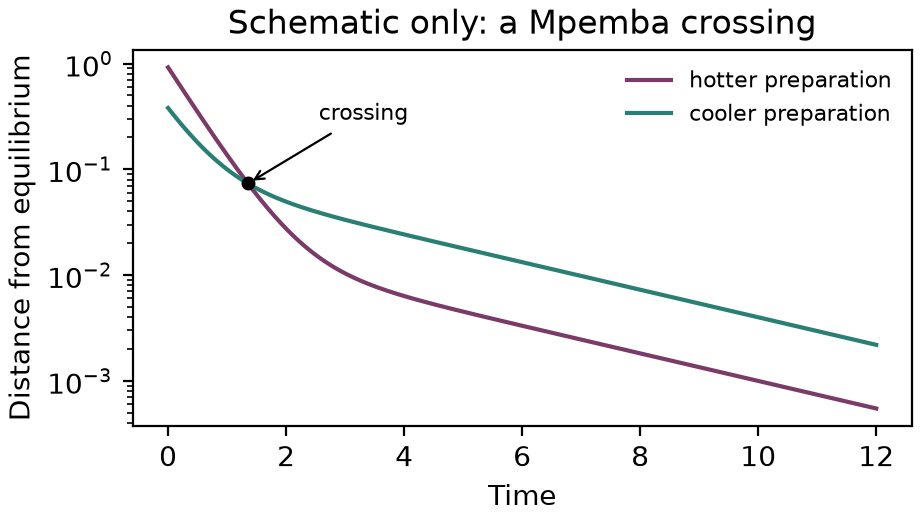
\includegraphics[width=.6\linewidth]{figures/schematic_crossing.png}
\caption{Schematic only (illustrative sums of two exponentials, not data or a model from this paper): the distance from equilibrium of a hotter and a cooler preparation relaxing in the same bath. The hotter curve starts higher but has a smaller slow-mode amplitude, so the curves cross. Proposition~\ref{prop:superohmic} certifies such a crossing for a concrete model.}
\label{fig:schematic}
\end{figure}
Figure~\ref{fig:schematic} sketches the situation. Three kinds of statement about such curves are common, and we keep them apart.
\begin{itemize}
\item \emph{Weak (slow-mode) effect} \cite{KlichRaz2019}: at late times each curve is dominated by the slowest relaxation mode, with an amplitude fixed by the preparation. The weak effect is an inversion of these amplitudes: the hotter preparation has the smaller slow-mode amplitude. It implies a crossing at some late time.
\item \emph{Strong effect} \cite{KlichRaz2019}: the slow-mode amplitude vanishes exactly at some preparation temperature, so that preparation relaxes exponentially faster. We call this nontrivial \emph{strong cancellation}.
\item \emph{All-time order}: the curves do not cross at any time, for a stated distance measure. This is the strongest exclusion and the one we aim for. It rules out the weak effect and also transient crossings at early or intermediate times.
\end{itemize}

\subsection{Background}
Lu and Raz framed the Mpemba effect and its inverse for Markov jump processes: a preparation farther from equilibrium can later be closer, measured by a distance function on distributions \cite{LuRaz2017}. Klich, Raz, Hirschberg and Vucelja then separated the weak and strong effects described above and counted strong effects with the Mpemba index \cite{KlichRaz2019}. Kumar and Bechhoefer observed exponentially faster cooling in a colloidal system \cite{Kumar2020}, and Walker and Vucelja related the effect to potential shape and phase transitions for overdamped Langevin particles \cite{Walker2021}. Exclusion results followed for special structures. Complete-graph Metropolis dynamics shows no Mpemba effect, whereas near-complete graphs can \cite{Klich2019}, and monotone-coupling hypotheses give a no-Mpemba theorem for many-body systems \cite{Ohga2024}. General comparison frameworks now cover thermomajorization \cite{Vu2025} and resource theories \cite{Summer2026}. Most recently, three-level necessary conditions on rates have been applied to $N$-level systems and bath spectra \cite{Avitan2026}, and four-level anomalies absent from all triplets have been constructed \cite{Gelbwaser2026}.

The closest antecedent is the work of Avitan, Factor and Gelbwaser-Klimovsky \cite{Avitan2026}. Using the slow-mode criterion, they already exclude the slow-mode (weak) Mpemba effect for sub-Ohmic, Ohmic and super-Ohmic spectra with exponent $s\le2$ in their parametrisation. Their $N$-level statement is proved at zero bath temperature, when every triplet strongly violates their three-level conditions; at positive bath temperature it is a conjecture supported by numerics up to seven levels, and the $s\le2$ exclusion is analytic in the high- and low-temperature limits and numerical in between. So the physical message ``such baths do not give a slow-mode Mpemba effect'' is not new here. We do not claim that their class of spectra coincides with our class of concave jump weights; the two are stated in different rate conventions (Sec.~\ref{sec:baths}). What this paper adds, for complete-graph rates with a common jump weight, is: (i) a proof at every finite bath temperature, for every number of levels and every spectrum, without spectral simplicity; (ii) order at all times rather than only of slow-mode amplitudes; (iii) the same conclusion for a family of divergences and for common schedules of noncommuting stages; and (iv) an exact necessity direction: if the weight is not concave, cone preservation fails for some spectrum and bath temperature. Point (iv) concerns the cone, not the existence of a crossing.

The mathematical ingredients are established. Increasing-in-mean inequalities supply the Gibbs comparison \cite{Biernacki1951,Dragomir2004}; stochastic orders, stochastic monotonicity and invariant cones are standard tools for Markov operators \cite{Shaked2007,Daley1968,KeilsonKester1977,Massey1987,Lorek2012}. The preparation-temperature derivative of relative entropy has already been expressed through a covariance by Ohga, Hayakawa and Ito \cite[Appendix B]{Ohga2024}. Our finite-time theorem combines that calculus with a particular cone's closure under increasing concave functions. We do not claim a new divergence framework: thermomajorization \cite{Vu2025}, resource-theoretic treatments \cite{Summer2026}, and the operator-convex kernel comparison of Salazar \cite{Salazar2026} address broader or different comparisons. Table~\ref{tab:position} summarises the boundaries.

\begin{table}[tb]
\centering\small
\caption{Contribution boundaries relative to the closest antecedents. Each added conclusion retains the hypotheses stated in the corresponding theorem.}
\label{tab:position}
\begin{tabular}{>{\raggedright\arraybackslash}p{.24\linewidth}>{\raggedright\arraybackslash}p{.33\linewidth}>{\raggedright\arraybackslash}p{.35\linewidth}}
\toprule Antecedent & Established scope & Additional conclusion here\\\midrule
Metropolis exclusion \cite{Klich2019} & Complete-graph Metropolis rates: no Mpemba effect; effect possible on near-complete graphs & Concave effective weights; finite-time selected divergences and common schedules\\[3pt]
Three-level necessary conditions \cite{Avitan2026} & Slow-mode exclusion for $s\le2$ spectra: proved at zero bath temperature (strong violation) and in high/low-temperature limits, numerical otherwise & All bath temperatures, $N$ and spectra for complete-graph common coupling; all-time order for a divergence family and schedules; exact necessity for cone preservation\\[3pt]
Monotone coupling \cite{Ohga2024} & Order-compatible dynamics; KL derivative/covariance identity & Prefix-cone sign criterion applicable to an explicit non-monotone-coupling example\\[3pt]
Four-state collective anomaly \cite{Gelbwaser2026} & A full anomaly without actual triplet anomalies & Every fixed $N$; all proper induced subsystems exclude the slow anomaly\\[3pt]
Thermomajorization and Petz kernels \cite{Vu2025,Salazar2026} & General comparisons across divergence families & A sufficient dynamical condition for Gibbs preparations in a specified family\\
\bottomrule
\end{tabular}
\end{table}

\subsection{Main results in plain words}
\begin{enumerate}[label=\arabic*.]
\item \textbf{A test for all-time order} (Theorem~\ref{thm:metric}). If the dynamics and its time reverse both keep the cone $\C$ of Sec.~\ref{sec:cone} inside itself, cooling preparations stay ordered at every time in relative entropy (both orientations), squared Hellinger distance and R\'enyi divergences of order $0<\alpha\le2$. The same holds for any common sequence of such dynamics (Corollary~\ref{cor:protocol}).
\item \textbf{Which baths pass the test} (Theorem~\ref{thm:concavity}, Proposition~\ref{prop:baths}). For complete-graph bosonic population dynamics with a common coupling, the test holds for every spectrum and bath temperature exactly when the spontaneous jump weight $J$ is concave. Ohmic, Drude--Lorentz and sub-Ohmic weights are concave below explicit cutoff thresholds; super-Ohmic weights are not.
\item \textbf{A certified crossing beyond the class} (Proposition~\ref{prop:superohmic}). For the super-Ohmic weight $J(d)=d^3$ on four equally spaced levels, the test fails and the relative entropies of two cooling preparations do cross.
\item \textbf{Total variation is a real exception} (Proposition~\ref{prop:TV}). A five-state system that passes the test still shows a short, small total-variation reversal, certified by exact interval arithmetic.
\item \textbf{Small subsystems cannot certify a large one} (Theorem~\ref{thm:hierarchy}). For every $N\ge4$ there is an $N$-level system with a slow-mode inversion and a total-variation crossing, although no proper induced subsystem has a slow-mode inversion.
\end{enumerate}

\subsection{Roadmap}
Section~\ref{sec:cone} introduces the Gibbs preparations, the distance measures and the cone, and places them in the theory of stochastic orders. Section~\ref{sec:metric} proves the finite-time test and lists the divergences it covers. Section~\ref{sec:physical} classifies bosonic jump weights, applies the result to standard bath spectral densities and gives the certified super-Ohmic crossing. Section~\ref{sec:tv} gives the total-variation boundary example. Section~\ref{sec:hierarchy} constructs the subsystem hierarchy. Section~\ref{sec:discussion} collects the scope and limits in one place. The appendices contain the certificate prescriptions, the proper-subsystem analysis and the derivations of the main matrix formulas.

\section{Thermal preparations and an observable cone}\label{sec:cone}
Fix $N\ge2$, strictly ordered energies $E_1<\cdots<E_N$, and a finite inverse bath temperature $\beta_b>0$. Define
\begin{equation}
 p_{\beta,i}=\frac{e^{-\beta E_i}}{Z(\beta)},\qquad
 Z(\beta)=\sum_i e^{-\beta E_i},\qquad \pi=p_{\beta_b}.
 \label{eq:gibbs}
\end{equation}
All preparation inverse temperatures are finite and nonnegative. Cooling means $0\le\beta<\beta_b$ (a preparation hotter than the bath relaxes by cooling); heating means $\beta>\beta_b$ (a preparation colder than the bath relaxes by heating). Boltzmann's constant is included in $\beta=1/(k_BT)$. Displayed energies and times use fixed units $E_0$ and $\tau_0$, so inverse temperatures mean $\beta E_0$ and rates mean rates multiplied by $\tau_0$.

A row-generator $G$ acts on observables: $G_{ij}\ge0$ for $i\ne j$, $G\one=0$, and population columns evolve by $\dot p=G^Tp$. Reversibility means $\pi_iG_{ij}=\pi_jG_{ji}$.

\paragraph{Distances, modes and subsystems.} Distances to equilibrium are $f$-divergences, defined in Eq.~\eqref{eq:fdiv} below. The total variation distance is $\TV(p,\pi)=\frac12\sum_i|p_i-\pi_i|=\sum_{i:p_i>\pi_i}(p_i-\pi_i)$. For a reversible irreducible $G$ the nonzero eigenvalues are real and negative. If the one closest to zero, $-\gamma$, is simple, its eigenfunction $f$ (with $Gf=-\gamma f$, $\pi^Tf=0$) is the \emph{slow mode}, and $a(\beta)=p_\beta^Tf$ is the \emph{slow-mode amplitude} of the preparation (Eq.~\eqref{eq:slow}). The weak effect is an inversion of $|a|$, and strong cancellation is a zero of $a$ away from $\beta_b$. An \emph{induced subsystem} on a set of states keeps the off-diagonal rates between those states and recomputes the diagonal escape rates. It is not a marginal process or an effective generator obtained by eliminating states.

\paragraph{The cone.} Write
\begin{equation}
 \C=\left\{b\in\R^N:
 d_j(b):=b_j-\frac1{j-1}\sum_{i<j}b_i\ge0,
 \quad j=2,\ldots,N\right\}.
 \label{eq:cone}
\end{equation}
The arithmetic prefix means $\mu_k=k^{-1}\sum_{i\le k}b_i$ are nondecreasing exactly when $b\in\C$. Increasing observables belong to $\C$, but the cone is larger: individual components may decrease. Constants form $\C\cap(-\C)$, and adding a constant changes no $d_j$. The likelihood ratio $p_\beta/\pi$ of a cooling preparation increases with energy, so it lies in $\C$; the question is whether the dynamics keeps it there.

The objects in this section belong to the theory of stochastic orders \cite{Shaked2007}. The Gibbs family is ordered in the likelihood-ratio sense: for $\beta<\beta'$ the ratio $p_{\beta,i}/p_{\beta',i}\propto e^{(\beta'-\beta)E_i}$ increases with $E_i$, so $p_\beta$ dominates $p_{\beta'}$ in likelihood ratio and hence in the usual stochastic order. Vectors in $\C$ are the sequences that are increasing in mean in the sense of Chebyshev and Biernacki \cite{Biernacki1951,Dragomir2004}. Lemma~\ref{lem:gibbs} says that, for Gibbs families, the likelihood-ratio comparison extends from increasing observables to this larger cone. Requiring a Markov semigroup to preserve a cone of test functions is the classical notion of stochastic monotonicity: Daley studied chains whose kernels preserve the usual stochastic order \cite{Daley1968}, Keilson and Kester characterised monotone matrices and monotone continuous-time processes \cite{KeilsonKester1977}, and Massey gave generator conditions for orderings of Markov processes on partially ordered spaces \cite{Massey1987}. Our hypothesis is of this type, applied to the cone $\C$ rather than to increasing functions, and imposed on both the propagator and its $\pi$-adjoint.

\begin{lemma}[Gibbs comparison and composition]\label{lem:gibbs}
If $b\in\C$, then $\beta\mapsto p_\beta^Tb$ is nonincreasing on $[0,\infty)$, and strictly decreasing at every finite $\beta$ if $b$ is nonconstant. If $\phi$ is increasing and concave on an interval containing the components of $b$, then $\phi(b)\in\C$. For $b\in-\C$, the expectation inequality reverses and increasing convex $\phi$ preserve $-\C$.
\end{lemma}
\begin{proof}
\emph{Derivative as a covariance.} Since $\partial_\beta p_{\beta,i}=-p_{\beta,i}(E_i-p_\beta^TE)$, we have $\partial_\beta p_\beta^Tb=-\Cov_{p_\beta}(E,b)$.

\emph{Cut decomposition.} Write $E_i=E_1+\sum_{k<N}(E_{k+1}-E_k)\mathbf1_{\{i>k\}}$. By bilinearity,
\begin{equation}
 \Cov_{p_\beta}(E,b)=\sum_{k<N}(E_{k+1}-E_k)\Cov_{p_\beta}(\mathbf1_{\{i>k\}},b)
 =\sum_{k<N}(E_{k+1}-E_k)P_k(1-P_k)(R_k-L_k),
 \label{eq:cut}
\end{equation}
where $P_k=\sum_{i\le k}p_{\beta,i}$ and $L_k,R_k$ are the $p_\beta$-weighted means of $b$ on the prefix $\{1,\ldots,k\}$ and the tail $\{k+1,\ldots,N\}$. The second equality is the elementary identity $\Cov(\mathbf1_T,b)=P(T)P(T^c)(\bar b_T-\bar b_{T^c})$ for an event $T$ with conditional means $\bar b$.

\emph{Signs.} For positive decreasing weights $w_i$ (the Gibbs weights decrease with energy for $\beta\ge0$), summation by parts gives
\begin{equation}
 \sum_{i\le k}w_i(b_i-\mu_k)
 =\sum_{\ell<k}(w_\ell-w_{\ell+1})\ell(\mu_\ell-\mu_k)\le0,
 \label{eq:abel}
\end{equation}
because $\mu_\ell\le\mu_k$ for $\ell<k$ when $b\in\C$. Thus $L_k\le\mu_k$. Every later component satisfies $b_j\ge\mu_{j-1}\ge\mu_k$ for $j>k$, so $R_k\ge\mu_k$. Hence $R_k\ge\mu_k\ge L_k$, every term of Eq.~\eqref{eq:cut} is nonnegative, and $p_\beta^Tb$ is nonincreasing.

\emph{Strictness.} If $b$ is nonconstant, let $j$ be the first index with $b_j\ne b_1$. Then $d_j(b)=b_j-b_1\ne0$, so $b_j>b_1$. For the cut $k=j-1$ we have $L_k=b_1=\mu_k$, while every tail component is at least $\mu_k=b_1$ and the tail component $b_j$ is strictly larger with positive weight. So $R_k>L_k$, and the term with $E_{k+1}-E_k>0$ and $0<P_k<1$ is strictly positive.

\emph{Composition.} Monotonicity followed by Jensen's inequality gives
\begin{equation}
 \phi(b_j)\ge\phi\!\left(\frac1{j-1}\sum_{i<j}b_i\right)
 \ge\frac1{j-1}\sum_{i<j}\phi(b_i).
 \label{eq:jensen}
\end{equation}
Both inequalities reverse for $b\in-\C$ and increasing convex $\phi$. Applying the first argument to $-b$ completes the proof.
\end{proof}
\takeaway{among Gibbs states, a hotter preparation gives a larger average to every observable in the cone, not only to increasing ones.}

\section{Finite-time divergence ordering}\label{sec:metric}
The next statement separates the ordering argument from a particular rate model. For $\langle u,v\rangle_\pi=\sum_i\pi_i u_iv_i$, consider a Markov operator on likelihood ratios satisfying
\begin{equation}
 K_{ij}\ge0,\quad K\one=\one,\quad \pi^TK=\pi^T,
 \qquad K^*=\diag(\pi)^{-1}K^T\diag(\pi).
 \label{eq:adjoint}
\end{equation}
The initial ratio and evolved population are
\begin{equation}
 r_{\beta,i}=p_{\beta,i}/\pi_i
 =\frac{Z(\beta_b)}{Z(\beta)}e^{(\beta_b-\beta)E_i},
 \qquad p^K_{\beta,i}=\pi_i(Kr_\beta)_i.
 \label{eq:ratio}
\end{equation}
All components remain positive. The hypotheses in Eq.~\eqref{eq:adjoint} are exactly what make $p^K$ a probability vector with the right fixed point:
\begin{equation}
 p^K\ge0,\qquad \one^Tp^K=\pi^TKr=\pi^Tr=1,\qquad r=\one\ \Longrightarrow\ p^K=\pi .
\end{equation}
On populations, $K$ acts as the column map $p\mapsto\diag(\pi)K\diag(\pi)^{-1}p$; $K$ itself should not be confused with the population transition matrix. For convex $f:(0,\infty)\to\R$ with $f(1)=0$, use
\begin{equation}
 D_f(p\Vert\pi)=\sum_i\pi_i f(p_i/\pi_i).
 \label{eq:fdiv}
\end{equation}
Affine multiples of $x-1$ do not affect this divergence.

\begin{theorem}[Two-adjoint thermal ordering]\label{thm:metric}
Suppose $K\C\subseteq\C$ and $K^*\C\subseteq\C$.
\begin{enumerate}[label=(\roman*)]
\item If $f$ is differentiable and $f'$ is increasing and concave, then
\begin{equation}
 \partial_\beta D_f(p^K_\beta\Vert\pi)\le0,
 \qquad 0\le\beta\le\beta_b.
 \label{eq:cool}
\end{equation}
\item If $f'$ is increasing and convex, then
\begin{equation}
 \partial_\beta D_f(p^K_\beta\Vert\pi)\ge0,
 \qquad \beta\ge\beta_b.
 \label{eq:heat}
\end{equation}
\item If $K$ is invertible and $f'$ is strictly increasing, the respective inequalities are strict for $\beta\ne\beta_b$. The derivative is zero at $\beta_b$.
\end{enumerate}
\end{theorem}
\begin{proof}
Differentiate at fixed $K,\pi,E$. Moving $K$ across the weighted inner product yields
\begin{align}
 \partial_\beta D_f(p^K_\beta\Vert\pi)
 &=\langle f'(Kr_\beta),K\partial_\beta r_\beta\rangle_\pi\nonumber\\
 &=\sum_i p'_{\beta,i}[K^*f'(Kr_\beta)]_i\nonumber\\
 &=-\Cov_{p_\beta}\!\left(E,K^*f'(Kr_\beta)\right).
 \label{eq:mainidentity}
\end{align}
The KL instance of this derivative/covariance approach is an antecedent \cite{Ohga2024}. The sufficient sign condition here follows from three steps. For cooling, $r_\beta\in\C$ because its components increase with energy. Cone preservation gives $Kr_\beta\in\C$; Lemma~\ref{lem:gibbs} gives $f'(Kr_\beta)\in\C$; adjoint cone preservation gives $K^*f'(Kr_\beta)\in\C$. Its covariance with energy is nonnegative by the same lemma. Heating uses $-\C$ and the convex composition statement.

Away from $\beta_b$, the initial ratio is nonconstant. An invertible operator fixing constants cannot turn a nonconstant vector into a constant. Strictly increasing $f'$ also preserves nonconstancy. Apply this successively to $K,f',K^*$ and use the strict Gibbs comparison. At equilibrium the resulting observable is the constant $f'(1)\one$.
\end{proof}

\takeaway{if the dynamics and its time reverse never push an ``increasing-on-average'' observable out of the cone, a hotter cooling preparation stays farther from equilibrium at every time, for every divergence whose generator has an increasing concave derivative.}

The next statement is a corollary of the closure of the cone-preserving class under products and adjoints; we do not present it as a separate result.
\begin{corollary}[Reversible evolution and common schedules]\label{cor:protocol}
Suppose $G_1,\ldots,G_s$ are reversible with respect to the same $\pi$ and each $e^{tG_k}$ preserves $\C$. For arbitrary finite durations $t_k\ge0$, Theorem~\ref{thm:metric} applies at every time of the common prescribed schedule. It is strict away from equilibrium whenever $f'$ is strictly increasing.
\end{corollary}
\begin{proof}
Set $P_k=e^{t_kG_k}$. Each $P_k$ is self-adjoint in $\langle\cdot,\cdot\rangle_\pi$ by reversibility. The row-distribution transition product is $P_1\cdots P_s$, whereas its likelihood-ratio operator and adjoint are
\begin{equation}
 K=P_s\cdots P_1,\qquad K^*=P_1\cdots P_s.
 \label{eq:protocol}
\end{equation}
At an intermediate time, during stage $j$ after an elapsed time $0\le\tau\le t_j$ in that stage, the operators are
\begin{equation}
 K(t)=e^{\tau G_j}P_{j-1}\cdots P_1,\qquad K(t)^*=P_1\cdots P_{j-1}e^{\tau G_j}.
\end{equation}
Every factor preserves $\C$, satisfies Eq.~\eqref{eq:adjoint} and is invertible. Both products therefore satisfy the theorem at every $t$.
\end{proof}

The stages need not commute and the total transition product need not be reversible. The same schedule must act on both preparations. This result does not compare different controls chosen for a fixed preparation, as in barrier-optimisation protocols \cite{Wang2026}. The bath, energy levels and ordering remain fixed here.

\subsection{Standard measures covered by the theorem}
For $C^3$ generators, convexity means $f''\ge0$; the additional cooling condition is $f'''\le0$, and the heating condition is $f'''\ge0$. Table~\ref{tab:metrics} gives familiar examples. In particular,
\begin{equation}
 \KL(p\Vert\pi)=\beta_b\{\mathcal F_{\beta_b}(p)-\mathcal F_{\beta_b}(\pi)\},
 \quad \mathcal F_{\beta_b}(p)=\sum_i p_iE_i+\beta_b^{-1}\sum_i p_i\log p_i.
\end{equation}
Thus the cooling result orders excess nonequilibrium free energy at every finite time.

\begin{table}[tb]
\centering\small
\caption{Guaranteed ordering under Theorem~\ref{thm:metric}. ``Cooling'' means increasing $\beta$ towards $\beta_b$ decreases the divergence; ``heating'' means increasing $\beta$ away from $\beta_b$ increases it.}
\label{tab:metrics}
\begin{tabular}{>{\raggedright\arraybackslash}p{.32\linewidth}>{\raggedright\arraybackslash}p{.38\linewidth}>{\raggedright\arraybackslash}p{.19\linewidth}}
\toprule Measure & Generator $f(x)$ & Guaranteed side\\\midrule
Forward relative entropy & $x\log x-x+1$ & Cooling\\
Reverse relative entropy & $x-1-\log x$ & Cooling\\
Squared Hellinger, $\frac12\sum_i(\sqrt{p_i}-\sqrt{\pi_i})^2$ & $\frac12(\sqrt x-1)^2$ & Cooling\\
Half Pearson chi-square & $\frac12(x-1)^2$ & Both\\
Power divergence $\mathcal P_\alpha$ & Eq.~\eqref{eq:power} & Cooling $\alpha\le2$; heating $\alpha\ge2$\\
Total variation & $\frac12|x-1|$ & Not guaranteed (Proposition~\ref{prop:TV})\\
\bottomrule
\end{tabular}
\end{table}

In the standard power-divergence family \cite{Cressie1984}, with index shifted by one from the original convention, put
\begin{equation}
 f_\alpha(x)=\frac{x^\alpha-\alpha x+\alpha-1}{\alpha(\alpha-1)},
 \quad f_\alpha''(x)=x^{\alpha-2},\quad
 f_\alpha'''(x)=(\alpha-2)x^{\alpha-3}.
 \label{eq:power}
\end{equation}
The continuous limits at $\alpha=1,0$ are forward and reverse KL. Consequently $\mathcal P_\alpha=D_{f_\alpha}$ is ordered for cooling at every real $\alpha\le2$ and for heating at every $\alpha\ge2$. For $\alpha>0$, R\'enyi divergence is the strictly increasing function
\begin{equation}
 D_\alpha^{\mathrm R}(p\Vert\pi)
 =\frac{\log[1+\alpha(\alpha-1)\mathcal P_\alpha(p\Vert\pi)]}{\alpha-1},
 \qquad
 \frac{\partial D_\alpha^{\mathrm R}}{\partial\mathcal P_\alpha}
 =\frac{\alpha}{1+\alpha(\alpha-1)\mathcal P_\alpha}>0.
 \label{eq:renyi}
\end{equation}
It inherits cooling order for $0<\alpha\le2$ and heating order for $\alpha\ge2$, with the usual $\alpha=1$ limit. R\'enyi order zero is not reverse KL: it vanishes for full-support distributions.

There is also a family-wide classical consequence, which we state with its hypotheses. Let $f:(0,\infty)\to\R$ be operator convex; such functions are real analytic on $(0,\infty)$, so $f''(1)$ is finite. Remove the affine part so that $f(1)=f'(1)=0$; this does not change $D_f$. If $f$ is not identically zero, then $f''(1)>0$, and we fix the scale by $f''(1)=2$. One standard form of the integral representation of operator convex functions on $(0,\infty)$ (see reference~\cite{Hiai2017} and references therein; the same kernels appear in reference~\cite{Salazar2026}) then reads
\begin{equation}
 f(x)=\int_{[0,1]}g_\lambda(x)\,d\nu(\lambda),
 \label{eq:opconvex}
\end{equation}
with a positive measure $\nu$ on the closed interval $[0,1]$, endpoint atoms allowed: $\lambda=1$ gives the $\chi^2$ kernel $(x-1)^2$ and $\lambda=0$ gives $(x-1)^2/x$. Here
\begin{equation}
 g_\lambda(x)=\frac{(x-1)^2}{(1-\lambda)x+\lambda},\quad0\le\lambda\le1,
 \qquad
 g_\lambda'''(x)=-\frac{6(1-\lambda)}{[(1-\lambda)x+\lambda]^4}\le0.
 \label{eq:petz}
\end{equation}
Since $g_\lambda''(1)=2$ for every $\lambda$, the normalisation $f''(1)=2$ is exactly the statement that $\nu$ is a probability measure. Their second derivatives $g_\lambda''(x)=2/[(1-\lambda)x+\lambda]^3$ are positive. Each scalar kernel, and hence every positive mixture, obeys the cooling order. This concerns the population reduction of the Petz family; it does not prove a statement for noncommuting density matrices. Nor does it cover every scalar convex $f$. Total variation has generator $|x-1|/2$, whose derivative has neither required global curvature. Thermomajorization requires the stronger all-convex-$f$ comparison \cite{Vu2025}. If one prefers not to rely on Eq.~\eqref{eq:opconvex}, the conclusion still holds for every family listed in Table~\ref{tab:metrics}, which was checked by direct differentiation above.

The asymmetry between the guaranteed sides in Table~\ref{tab:metrics} is consistent with, but distinct from, the heating--cooling asymmetry reported for thermodynamically equidistant quenches \cite{Lapolla2020,VanVu2021,Ibanez2024}. Those works compare the speed of heating and cooling from preparations at equal divergence, and Van Vu and Hasegawa show that heating is faster for every two-state system but not universally for more levels \cite{VanVu2021}. Theorem~\ref{thm:metric} instead compares two preparations on the same side of the bath and says nothing about relative speeds.

\section{An exact physical class: concave bosonic jump weights}\label{sec:physical}
Consider the complete-graph population rates
\begin{equation}
 G_{ij}=\frac{J(|E_i-E_j|)}{e^{\beta_b|E_i-E_j|}-1}
       +\mathbf1_{E_i>E_j}J(|E_i-E_j|),\qquad i\ne j,
 \label{eq:boson}
\end{equation}
with diagonal entries fixed by row sums. Thus the downward rate is $J(d)[n_b(d)+1]$ and the upward rate is $J(d)n_b(d)$, with the Bose factor $n_b(d)=1/(e^{\beta_bd}-1)$ written explicitly; $J$ is the spontaneous (zero-temperature) emission weight. The effective weight $J$ includes any common frequency dependence of the transition matrix element. A common pairwise coupling prefactor can be absorbed in $J$. Equation~\eqref{eq:boson} does not permit an independently chosen matrix element for each pair. It satisfies detailed balance with Eq.~\eqref{eq:gibbs}.

\begin{theorem}[Uniform-in-$(N,\beta_b)$ cone characterisation]\label{thm:concavity}
Fix $D>0$ and a continuous nonnegative function $J$ on $[0,D]$. The following are equivalent:
\begin{enumerate}[label=(\roman*)]
\item $J$ is concave on $[0,D]$.
\item For every finite strictly ordered spectrum of width at most $D$ and every finite $\beta_b>0$, the generator in Eq.~\eqref{eq:boson} satisfies $e^{tG}\C\subseteq\C$ for all $t\ge0$.
\end{enumerate}
\end{theorem}
Condition (ii) quantifies over all numbers of levels and all spectra \emph{and} over arbitrarily cold baths, jointly. The necessity proof below uses both: many clustered levels and a low bath temperature. At a fixed number of levels, or at a fixed bath temperature, concavity is sufficient but not necessary. For example, $J(d)=1+d^2$ is convex on $[0,1]$, yet every three-level spectrum preserves the cone at every bath temperature (Sec.~\ref{sec:separators}). Its first exact failure we exhibit uses six levels at $\beta_b=10\log2$. A floating-point search (numerical, not certified) found no failure with at most ten levels at $\beta_b=1/4$, $1/2$ and $1$; failures appeared only for clustered spectra with at least twelve levels.

\takeaway{for this standard class of bath-driven population dynamics, the test of Theorem~\ref{thm:metric} is passed by every spectrum and every bath temperature exactly when the spontaneous emission weight bends downwards (is concave) as a function of frequency.}

\subsection{Coordinates for cone preservation}
For $j=2,\ldots,N$, let $u^{(j)}$ have entries $-1$ before $j$, entry $j-1$ at $j$, and zero afterwards. These orthogonal Helmert contrasts satisfy $\|u^{(j)}\|^2=j(j-1)$ and $(u^{(j)})^Tb=(j-1)d_j(b)$. Modulo constants,
\begin{equation}
 b=\sum_{j=2}^N\frac{d_j(b)}{j}u^{(j)},\qquad
 H_{ij}=\frac{(u^{(i)})^TGu^{(j)}}{(i-1)j},\quad i,j=2,\ldots,N.
 \label{eq:helmert}
\end{equation}
Thus $d(Gb)=Hd(b)$ (Appendix~\ref{app:derivations}). The standard positive-semigroup criterion states that $e^{tH}$ preserves the nonnegative orthant exactly when $H$ is Metzler, meaning $H_{ij}\ge0$ for $i\ne j$. Indeed, if $H$ is Metzler, choose $c$ so $H+cI$ is entrywise nonnegative. The exponential series gives $e^{tH}=e^{-ct}e^{t(H+cI)}\ge0$. Conversely, if $e^{tH}\ge0$ for every $t\ge0$, its off-diagonal derivative at zero gives $H_{ij}=\lim_{t\downarrow0}(e^{tH})_{ij}/t\ge0$. This equivalence transports directly to $\C$. It is an application of established invariant-cone and monotone-matrix methods \cite{KeilsonKester1977,Massey1987,Lorek2012}.

\subsection{Sufficiency}
Split $G=S+W$, where $S$ is the symmetric thermal part with off-diagonal rates
\begin{equation}
 h(d)=\frac{J(d)}{e^{\beta_b d}-1},
\end{equation}
and $W$ is the spontaneous-emission part, with only downward rates $W_{ij}=J(E_i-E_j)$ for $i>j$. Concavity and $J(0)\ge0$ imply that $J(d)/d$ is nonincreasing. The factor $d/(e^{\beta_b d}-1)$ is positive and strictly decreasing, so $h$ is nonincreasing. Direct expansion of Eq.~\eqref{eq:helmert} (Appendix~\ref{app:derivations}) gives, for $2\le i<j\le N$,
\begin{align}
 H^S_{ij}
 &=h(E_j-E_i)-\frac1{i-1}\sum_{k<i}h(E_j-E_k)\nonumber\\
 &\quad+\frac1j\sum_{\ell>j}\left[h(E_\ell-E_i)
       -\frac1{i-1}\sum_{k<i}h(E_\ell-E_k)\right]\ge0.
 \label{eq:thermalH}
\end{align}
Every comparison uses the smaller gap in the first term. Symmetry of $S$ gives
\begin{equation}
 H^S_{ji}=\frac{(i-1)j}{(j-1)i}H^S_{ij}\ge0.
\end{equation}

The upper off-diagonal entries of $H^W$ vanish. For a fixed column $j$, define
\begin{equation}
 S_j=\sum_{\ell<j}J(E_j-E_\ell),\quad
 F_j(x)=(j-1)J(x-E_j)-\sum_{\ell<j}J(x-E_\ell),\quad x\ge E_j.
\end{equation}
For a concave function, fixed-length increments $J(z+a)-J(z)$ are nonincreasing in $z$ (Lemma~\ref{lem:increments}). Therefore $F_j$ is nondecreasing and $F_j(E_j)+S_j=(j-1)J(0)\ge0$. For $i>j$, multiplication in Eq.~\eqref{eq:helmert} yields
\begin{align}
 (i-1)jH^W_{ij}
 &=j\{F_j(E_i)+S_j\}
   +\sum_{k=j+1}^{i-1}\{F_j(E_i)-F_j(E_k)\}\ge0.
 \label{eq:downH}
\end{align}
Hence $H=H^S+H^W$ is Metzler, proving sufficiency. The downward limit separately preserves the cone.

\subsection{Necessity with its exact quantifiers}
\begin{lemma}[Increment characterisation of concavity]\label{lem:increments}
A continuous function $J$ on $[0,D]$ is concave if and only if, for every $\Delta\in(0,D)$, the increment $I_\Delta(z)=J(z+\Delta)-J(z)$ is nonincreasing on $[0,D-\Delta]$.
\end{lemma}
\begin{proof}
For $0\le z<z'\le D-\Delta$, rearrangement gives the identity
\begin{equation}
 I_\Delta(z)-I_\Delta(z')=[J(z')-J(z)]-[J(z'+\Delta)-J(z+\Delta)].
\end{equation}
If $J$ is concave, chord slopes decrease from left to right: for $a<b\le c<e$, the slope of $J$ on $[a,b]$ is at least its slope on $[c,e]$. If $z'-z\le\Delta$, apply this to $[z,z']$ and $[z+\Delta,z'+\Delta]$, two intervals of equal length with the first to the left; the right-hand side of the identity is then nonnegative. If $z'-z>\Delta$, apply it instead to $[z,z+\Delta]$ and $[z',z'+\Delta]$, which gives $I_\Delta(z)\ge I_\Delta(z')$ directly. Conversely, if every $I_\Delta$ is nonincreasing, then $I_\Delta(z)\ge I_\Delta(z+\Delta)$ is $J(z+\Delta)\ge\frac12[J(z)+J(z+2\Delta)]$, i.e.\ midpoint concavity. A continuous midpoint-concave function is concave.
\end{proof}

If a continuous $J$ is not concave, Lemma~\ref{lem:increments} gives $\Delta>0$ and $0\le x<y$, with $\Delta+y\le D$, such that
\begin{equation}
 I_\Delta(y)>I_\Delta(x),\qquad I_\Delta(z)=J(z+\Delta)-J(z).
 \label{eq:increment}
\end{equation}
Take $N=M+3$ energies consisting of $0,\Delta$, then $M$ levels near $\Delta+x$, then $\Delta+y$. In the coalescing middle-level limit, direct evaluation of Eq.~\eqref{eq:downH} with $j=2$, $i=N$ (Appendix~\ref{app:derivations}) gives
\begin{equation}
 H^W_{N2}\longrightarrow
 \frac{2J(\Delta)+M I_\Delta(x)-(M+2)I_\Delta(y)}{2(M+2)}.
 \label{eq:necessity}
\end{equation}
The numerator equals $2[J(\Delta)-I_\Delta(y)]-M[I_\Delta(y)-I_\Delta(x)]$, so it is negative for the explicit choice
\begin{equation}
 M=1+\max\left\{0,\left\lfloor\frac{2[J(\Delta)-I_\Delta(y)]}{I_\Delta(y)-I_\Delta(x)}\right\rfloor\right\}.
 \label{eq:Mchoice}
\end{equation}
Strictness and continuity allow a cluster of distinct intermediate energies retaining the sign. If $x=0$, put that cluster just above $\Delta$; one-sided continuity suffices. Fix these distinct energies before lowering the bath temperature. Every nonzero gap is then fixed, and $H^S\to0$ as $\beta_b\to\infty$. The same negative off-diagonal entry therefore persists at some finite bath temperature, contradicting cone preservation. This proves Theorem~\ref{thm:concavity}.

The necessity statement is universal over dimensions and spectra. It does not say that every nonconcave $J$ produces a thermal crossing for a given spectrum. The observable exposing cone failure need not increase with energy, and changing energies also changes the gap-dependent generator. Section~\ref{sec:superohmic} gives one nonconcave case where an actual crossing is certified.

\subsection{Consequences and exact scope separators}\label{sec:separators}
Theorems~\ref{thm:metric} and \ref{thm:concavity} give all-time cooling order for the divergences in Table~\ref{tab:metrics}, and for their stated positive transforms, for every concave $J$. Corollary~\ref{cor:protocol} permits a finite sequence of different concave $J_k$ at fixed energies and bath, with a common prescribed schedule. Figure~\ref{fig:thermal} illustrates a genuinely noncommuting example.

There is also an energy-distribution statement that does not depend on a divergence. For any increasing observable $b$, any $0\le\beta_h<\beta_c$, and any $t\ge0$,
\begin{equation}
 p_{\beta_h}^T e^{tG}b\ge p_{\beta_c}^T e^{tG}b.
 \label{eq:energyorder}
\end{equation}
Indeed, $e^{tG}b\in\C$ and Lemma~\ref{lem:gibbs} applies. Taking all energy-threshold indicators proves first-order stochastic ordering of the two evolving energy distributions. The preparations need not be on the same side of the bath. The same proof works for a common admissible schedule.

If $J$ is positive at every nonzero gap, every off-diagonal entry in Eq.~\eqref{eq:thermalH} is strictly positive. Perron--Frobenius theory applied to the Metzler quotient makes its spectral bound a simple eigenvalue with strictly positive $d$-coordinates. The quotient spectrum is the nonzero spectrum of $G$. Detailed balance and irreducibility make that spectral bound the simple slow eigenvalue. Lifting its quotient eigenvector and subtracting its stationary mean gives a genuine eigenfunction $f\in\C$ with $\pi^Tf=0$ and every $d_j(f)>0$. Its Gibbs amplitude $p_\beta^Tf$ is strictly decreasing and vanishes only at $\beta_b$. Thus its magnitude has conventional order on each side of the bath, excluding weak slow-mode inversion and nontrivial strong cancellation. For $N=2$ the single nonzero mode gives the same conclusion directly.

At zero bath temperature, when all excited states reach the ground, total variation from equilibrium is the survival probability $1-p_1(t)$. Its observable is increasing, so Eq.~\eqref{eq:energyorder} also excludes all-time total-variation reversal in this limit. This argument does not extend total variation automatically to a finite bath.

\begin{figure}[tb]
\centering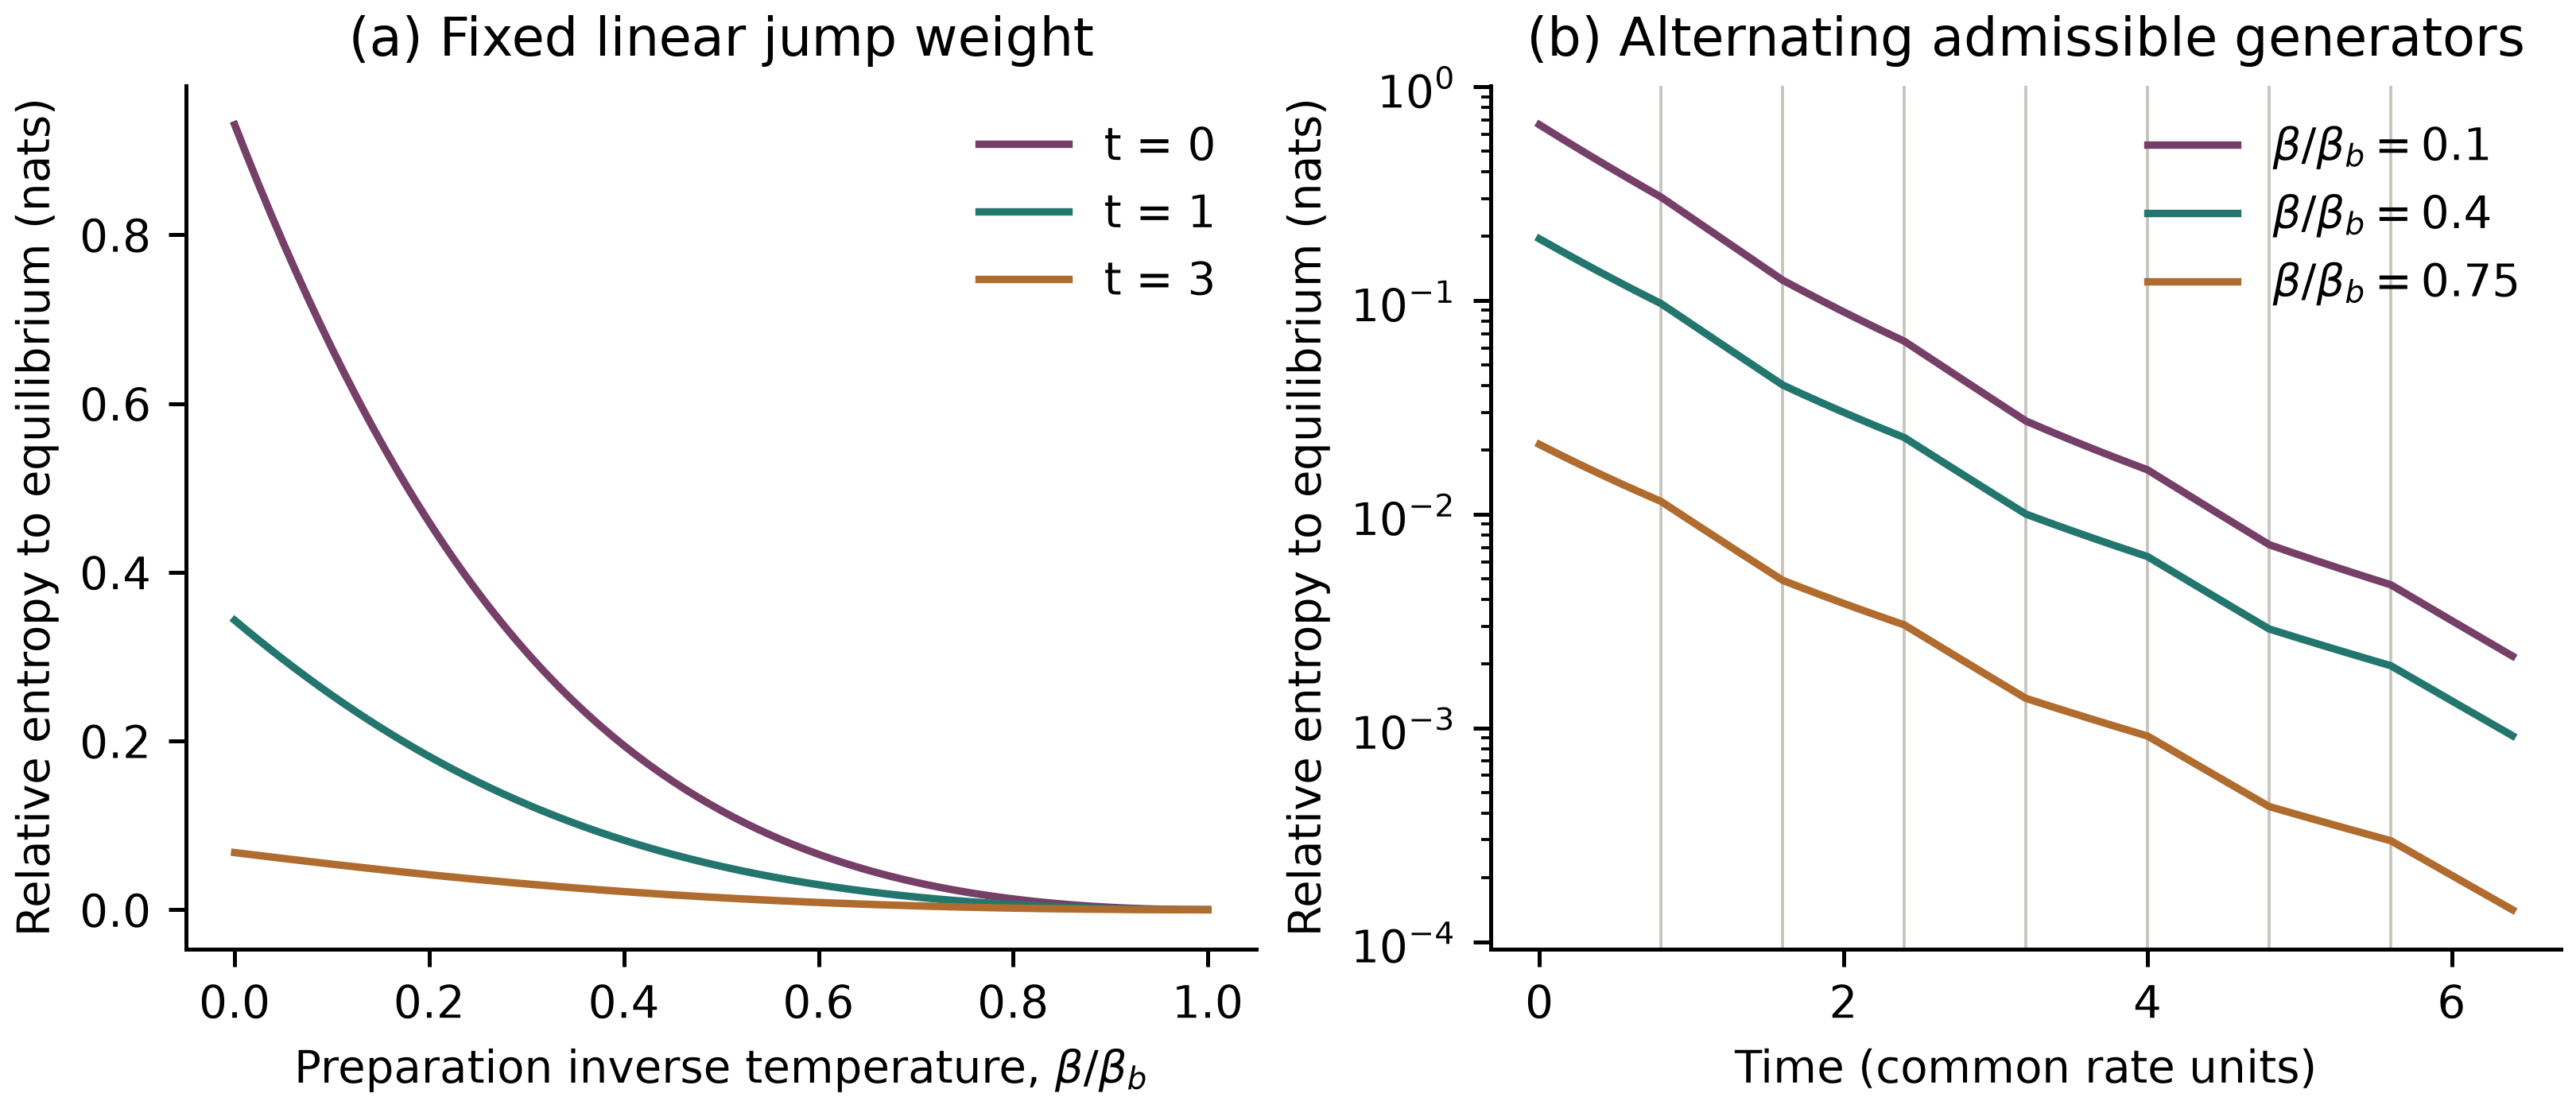
\includegraphics[width=\linewidth]{figures/thermal_order.png}
\caption{Finite-time relative-entropy ordering. Energies are $(0,1,2,4,7)$ and $\beta_b=\log2$. Each displayed generator is divided by its own maximum escape rate, defining two fixed matrices in common time units; the two weights are therefore not compared in a common physical time scale. (a) For $J_1(d)=d$, relative entropy decreases with preparation inverse temperature at each shown time. (b) The schedule alternates $J_1$ and $J_2(d)=1-e^{-\beta_b d}$ every $0.8$ time units. The three Gibbs preparations retain their order throughout. The generator commutator has Frobenius norm $0.1379$, so the schedule is not a commuting special case. The curves illustrate the theorem; they are not an optimisation or experimental dataset.}
\label{fig:thermal}
\end{figure}

In Figure~\ref{fig:thermal} each generator is normalised by its own maximum escape rate, so one time unit means a different physical time for $J_1$ and $J_2$. This does not affect the ordering statement, which holds for any durations.

The cone criterion differs from ordinary stochastic monotonicity on energy-ordered point masses. For $E=(0,1,2)$, $\beta_b=\log2$ and $J(d)=d$,
\begin{equation}
 G=\begin{pmatrix}-5/3&1&2/3\\2&-3&1\\8/3&2&-14/3\end{pmatrix},
 \qquad
 H=\begin{pmatrix}-23/6&1/3\\1/4&-11/2\end{pmatrix}.
 \label{eq:three}
\end{equation}
The initially higher point mass reaches the ground at rate $8/3$, exceeding the rate $2$ from the middle state. Thus ordinary stochastic monotonicity in the sense of Daley \cite{Daley1968} fails at small times, although all Gibbs preparations satisfy Eq.~\eqref{eq:energyorder}. On this complete graph, an energy-compatible order comparing every allowed transition must be the energy total order. The monotone-coupling hypotheses of reference~\cite{Ohga2024} therefore do not directly establish this example.

Nor can the all-dimension cone condition be replaced by a triplet check. Let $J(d)=1+d^2$ on $[0,1]$. For a zero-bath triplet with adjacent gaps $a,b$,
\begin{equation}
 H^W_{32}=\frac{J(a)+J(b)-J(a+b)}2
 =\frac{1-2ab}{2}\ge\frac14.
\end{equation}
Moreover $h(d)$ decreases on this interval at every positive bath: $J(d)/d=d+d^{-1}$ is nonincreasing for $d\le1$. Thus every such triplet preserves the cone at finite bath as well. In contrast, the distinct six-level spectrum
\begin{equation}
 E=(0,1/2,501/1000,502/1000,503/1000,1)
\end{equation}
has $H^W_{62}=-247/5000$. At $\beta_b=10\log2$, the thermal middle terms cancel and
\begin{equation}
 H^S_{62}=\frac35\left[\frac{5/4}{2^5-1}-\frac2{2^{10}-1}\right]
 =\frac{157}{6820},\qquad
 H_{62}=-\frac{44977}{1705000}<0.
 \label{eq:six}
\end{equation}
This is an exact finite-bath failure of cone preservation, with no minimal-dimension or thermal-crossing claim. Finally, at a fixed bath $J(d)=1-e^{-\beta_b d}$ gives downward rates $1$ and upward rates $e^{-\beta_b d}$ exactly. This is the known complete-graph Metropolis chain \cite{Klich2019}, recovered as a special case.

\subsection{Standard bath spectral densities}\label{sec:baths}
\emph{Convention.} For a weak-coupling (Born--Markov--secular) population model with one coupling operator of common pair matrix element $|g|^2$ and bath spectral density $\mathcal J(\omega)$, the downward and upward rates are $2\pi|g|^2\mathcal J(\omega)[n_b(\omega)+1]$ and $2\pi|g|^2\mathcal J(\omega)n_b(\omega)$. Comparing with Eq.~\eqref{eq:boson}, $J=2\pi|g|^2\mathcal J$, with $\hbar=1$. If a convention writes the rates with an extra power $\omega^k$ (for instance from the frequency dependence of a dipole matrix element), the results below apply to $\omega^k\mathcal J(\omega)$ instead. Named spectral densities in other papers must therefore be translated before comparison. In particular, Eq.~(5) of reference~\cite{Avitan2026} (arXiv version 1) reads $a_{kj}=f(\Delta)\propto\Delta^{s-1}e^{-\Delta/\Delta_c}\left[\frac{1}{e^{\beta_b\Delta}-1}+1\right]$. Comparing with the downward rate $J(\Delta)[n_b(\Delta)+1]$ of Eq.~\eqref{eq:boson} gives $J(\Delta)\propto\Delta^{s-1}e^{-\Delta/\Delta_c}$: their exponent $s$ equals our power-law exponent plus one (our exponent $s'$ in Proposition~\ref{prop:baths}(b) is $s'=s-1$), and their exclusion range $s\le2$ is not the same set as the concave weights below. For example, their Ohmic case $s=1$ corresponds to $J\propto e^{-d/\omega_c}$, which is concave on no interval (Proposition~\ref{prop:baths}(b) with $s=0$), and the cube law of Proposition~\ref{prop:superohmic} would correspond to their $s=4$, outside their range, so that example does not conflict with their exclusion. We do not claim a mapping between the two classes beyond this observation.

\begin{proposition}[Standard bath spectral densities]\label{prop:baths}
Let $\kappa>0$, $\omega_c>0$, $D>0$, and let $J$ be the jump weight of Eq.~\eqref{eq:boson} on $[0,D]$.
\begin{enumerate}[label=(\alph*)]
\item \emph{Pure power law} $J(d)=\kappa d^s$, $s\ge0$, with no cutoff factor on $[0,D]$ (for example a hard cutoff above $D$; a smooth cutoff changes the curvature and is treated in (b)--(d)). $J$ is concave on $[0,D]$ for every $D>0$ if $0\le s\le1$, and for no $D>0$ if $s>1$.
\item \emph{Exponential cutoff} $J(d)=\kappa d^se^{-d/\omega_c}$, $s\ge0$. $J$ is concave on $[0,D]$ if and only if $0<s\le1$ and
\begin{equation}
 D\le(s+\sqrt s)\,\omega_c .
 \label{eq:expthreshold}
\end{equation}
In particular the Ohmic case $s=1$ requires $D\le2\omega_c$. For $s=0$ and for every super-Ohmic $s>1$, $J$ is concave on no interval $[0,D]$.
\item \emph{Drude--Lorentz} $J(d)=\kappa\,\omega_c d/(d^2+\omega_c^2)$. $J$ is concave on $[0,D]$ if and only if $D\le\sqrt3\,\omega_c$.
\item \emph{Gaussian Ohmic cutoff} $J(d)=\kappa d\,e^{-d^2/\omega_c^2}$. $J$ is concave on $[0,D]$ if and only if $D\le\sqrt{3/2}\,\omega_c$.
\end{enumerate}
Nonnegative combinations of weights that are concave on $[0,D]$ remain concave on $[0,D]$.
\end{proposition}

\begin{proof}
All four weights are continuous and nonnegative on $[0,\infty)$ and smooth on $(0,\infty)$. A function continuous on $[0,D]$ and twice differentiable on $(0,D)$ is concave on $[0,D]$ if and only if $J''\le0$ on $(0,D)$: the forward direction is standard, and conversely $J''\le0$ makes $J'$ nonincreasing on $(0,D)$, so $J$ is concave on $(0,D)$ and, by continuity, on its closure. If $J''>0$ on a nonempty open subinterval of $(0,D)$, then $J$ is strictly convex there and hence not concave on $[0,D]$.

(a) $J''(d)=\kappa s(s-1)d^{s-2}$ for $d>0$, which is $\le0$ when $0\le s\le1$ and $>0$ when $s>1$.

(b) For $d>0$ and $y=d/\omega_c$, direct differentiation gives
\begin{equation}
 J''(d)=\kappa\,d^{s-2}e^{-d/\omega_c}\,Q_s(y),\qquad Q_s(y)=y^2-2sy+s(s-1),
 \label{eq:Qs}
\end{equation}
with roots $y_\pm=s\pm\sqrt s$. If $0<s\le1$, then $y_-=s-\sqrt s\le0<y_+$, so $Q_s<0$ on $(0,y_+)$ and $Q_s>0$ on $(y_+,\infty)$; thus $J''\le0$ on $(0,D)$ exactly when $D\le y_+\omega_c$. If $s>1$, then $0<y_-$ and $Q_s(0)=s(s-1)>0$, so $J''>0$ on $(0,y_-\omega_c)$. If $s=0$, $Q_0(y)=y^2>0$.

(c) Writing $c=\omega_c$, $J''(d)=-2\kappa c\,d(3c^2-d^2)/(d^2+c^2)^3$, which is $\le0$ on $(0,D)$ iff $D\le\sqrt3\,c$ and positive for $d>\sqrt3\,c$.

(d) $J''(d)=-(2\kappa d/\omega_c^2)\,(3-2d^2/\omega_c^2)\,e^{-d^2/\omega_c^2}$, which is $\le0$ on $(0,D)$ iff $D^2\le3\omega_c^2/2$.

Concavity on a fixed interval is preserved by nonnegative linear combinations.
\end{proof}

\begin{corollary}[Physical reading of Theorem~\ref{thm:concavity}]\label{cor:baths}
Let $D=E_N-E_1$ be the largest transition frequency of the spectrum.
\begin{enumerate}[label=(\roman*)]
\item \emph{Sufficiency.} If $J$ satisfies a concavity condition of Proposition~\ref{prop:baths} on $[0,D]$ (for example an Ohmic bath with $D\le2\omega_c$, a sub-Ohmic bath $s\in(0,1)$ with $D\le(s+\sqrt s)\omega_c$, or a Drude--Lorentz bath with $D\le\sqrt3\,\omega_c$), then for \emph{every} strictly ordered spectrum of width at most $D$ and every finite $\beta_b>0$ the conclusions of Theorem~\ref{thm:metric} hold at all times. Cooling Gibbs preparations retain their order in forward and reverse relative entropy (excess free energy), squared Hellinger distance and R\'enyi divergences of order $0<\alpha\le2$, and their energy distributions remain first-order stochastically ordered, Eq.~\eqref{eq:energyorder}. Since these weights are positive at every nonzero gap, slow-mode inversion and nontrivial strong cancellation are also excluded. By Corollary~\ref{cor:protocol}, the same holds for a common schedule switching among such weights at fixed energies and bath.
\item \emph{Necessity is existential.} If $J$ is not concave on $[0,D]$ (Ohmic beyond $2\omega_c$, Drude--Lorentz beyond $\sqrt3\,\omega_c$, and every super-Ohmic bath, including free-space dipole emission and three-dimensional acoustic phonons, $J\propto d^3$), Theorem~\ref{thm:concavity} only asserts that \emph{some} spectrum of width at most $D$ and \emph{some} finite bath temperature violate cone preservation. It does not assert that any given spectrum fails, nor that a thermal crossing occurs. Proposition~\ref{prop:superohmic} supplies an explicit super-Ohmic spectrum where both happen.
\end{enumerate}
\end{corollary}
\takeaway{in the complete-graph, common-coupling model, two cooling Gibbs preparations cannot cross in these measures at any time if the bath is Ohmic with cutoff frequency at least half the full spectral width (top level minus bottom level), Drude--Lorentz with cutoff at least $1/\sqrt3$ of that width, or a sub-Ohmic power law below its threshold; super-Ohmic baths are outside this guarantee.}

\subsection{A certified super-Ohmic crossing}\label{sec:superohmic}
\begin{proposition}[A super-Ohmic relative-entropy crossing]\label{prop:superohmic}
Take $J(d)=d^3$ in Eq.~\eqref{eq:boson}, energies $E=(0,1,2,3)$ and $e^{-\beta_b}=2/3$ ($\beta_b=\log\frac32$). Then
\begin{equation}
 G=\begin{pmatrix}
 -1878/95&2&32/5&216/19\\
 3&-57/5&2&32/5\\
 72/5&3&-97/5&2\\
 729/19&72/5&3&-5298/95
 \end{pmatrix},\qquad
 \pi=\tfrac1{65}(27,18,12,8),
 \label{eq:superG}
\end{equation}
and every off-diagonal entry of its cone quotient is negative,
\begin{equation}
 H=\begin{pmatrix}
 -1718/95&-1726/285&-472/95\\
 -1433/190&-492/19&-654/95\\
 -3224/285&-4024/285&-5924/95
 \end{pmatrix},
 \label{eq:superH}
\end{equation}
so $e^{tG}\C\not\subseteq\C$ for small $t>0$. For the cooling preparations $e^{-\beta_h}=9/10$ and $e^{-\beta_c}=4/5$ ($0<\beta_h<\beta_c<\beta_b$),
\begin{equation}
\begin{aligned}
 \KL(p_{\beta_h}(t)\Vert\pi)&>\KL(p_{\beta_c}(t)\Vert\pi)\quad\text{at}\ t\in\{0,\tfrac1{10},\tfrac15\},\\
 \KL(p_{\beta_h}(t)\Vert\pi)&<\KL(p_{\beta_c}(t)\Vert\pi)\quad\text{at}\ t\in\{\tfrac3{10},\tfrac25,\tfrac12\},
\end{aligned}
\end{equation}
so the forward relative entropies of two cooling Gibbs preparations cross at some $t\in(1/5,3/10)$.
\end{proposition}
\begin{proof}
All entries of $G$, $\pi$, $p_\beta$ and $H$ are rational and are checked by exact arithmetic, together with detailed balance and positivity of every rate. For $t>0$, the populations are enclosed by stochastic uniformisation at rate $R=56\ge\max_i|G_{ii}|$ with $161$ series terms and the geometric tail bound of Eq.~\eqref{eq:interval}; the largest component width is below $10^{-65}$. Writing $\KL(p\Vert\pi)=\sum_i\pi_i\phi(p_i/\pi_i)$ with $\phi(r)=r\log r-r+1$, each $\log r$ is enclosed by the series $2\operatorname{artanh}\frac{r-1}{r+1}$ with a rational geometric remainder, and $\phi$ is bounded on each ratio interval using that it decreases on $(0,1)$ and increases on $(1,\infty)$. The resulting rational enclosures are summarised in Table~\ref{tab:superohmic}; their signs prove the statement, and continuity in $t$ gives the crossing.
\end{proof}

\begin{table}[tb]
\centering\small
\caption{Rational-interval certificate for Proposition~\ref{prop:superohmic} ($J=d^3$, $E=(0,1,2,3)$, $e^{-\beta_b}=2/3$). Each enclosure agrees to at least twelve significant digits; six are shown. The ratio column is a certified lower bound. The last column gives certified rational bounds (decimals rounded outward) for $\KL(p_{\beta_h}(t)\Vert\pi)-\KL(p_{\beta_c}(t)\Vert\pi)$, whose signs prove Proposition~\ref{prop:superohmic}.}
\label{tab:superohmic}
\setlength{\tabcolsep}{3pt}\footnotesize\begin{tabular}{ccccc}
\toprule
$t$ & $\KL(p_{\beta_h}(t)\Vert\pi)$ & $\KL(p_{\beta_c}(t)\Vert\pi)$ & ratio cold/hot & hot $-$ cold, certified bounds\\\midrule
$0$ & $5.41264\times10^{-2}$ & $1.93991\times10^{-2}$ & $0.358$ & $[3.47273279998,\ 3.47273279999]\times10^{-2}$\\
$1/10$ & $4.85247\times10^{-5}$ & $2.20552\times10^{-5}$ & $0.454$ & $[2.64694826794,\ 2.64694826795]\times10^{-5}$\\
$1/5$ & $2.88684\times10^{-7}$ & $1.87865\times10^{-7}$ & $0.650$ & $[1.00819515073,\ 1.00819515074]\times10^{-7}$\\
$3/10$ & $1.92629\times10^{-9}$ & $4.57862\times10^{-9}$ & $2.376$ & $[-2.65233420602,\ -2.65233420601]\times10^{-9}$\\
$2/5$ & $2.51753\times10^{-11}$ & $2.33165\times10^{-10}$ & $9.261$ & $[-2.07989519898,\ -2.07989519897]\times10^{-10}$\\
$1/2$ & $9.71389\times10^{-13}$ & $1.36083\times10^{-11}$ & $14.009$ & $[-1.26368973414,\ -1.26368973413]\times10^{-11}$\\
\bottomrule
\end{tabular}
\end{table}

\emph{What is certified and what is numerical.} Certified by exact rational arithmetic: the rates, detailed balance, the negative off-diagonal entries of $H$ (cone failure), and the signs of the relative-entropy difference at the six listed times, hence a crossing in $(1/5,3/10)$. The same spectrum and bath with the Ohmic weight $J(d)=d$ give a Metzler quotient, so Theorem~\ref{thm:metric} forbids any such crossing there; the crossing is therefore attributable to the convex jump weight. Numerical only (double precision, not part of the certificate): the crossing is at $t\approx0.2423$, about $3.4$ slow relaxation times ($\gamma_{\rm slow}\approx14.12$). With the slow eigenfunction normalised by $\pi^Tf=0$ and $\|f\|_2=1$ (sign fixed by $f_2-f_1>0$), the signed slow amplitudes $a(\beta)=p_\beta^Tf$ are $3.9\times10^{-3}$, $-8.2\times10^{-4}$ and $-3.2\times10^{-3}$ at $e^{-\beta}=1,\,9/10,\,4/5$. The reversed order is thus a slow-mode inversion that persists at late times, and the sign change of $a$ on $(0,\beta_h)$ indicates a strong-effect preparation temperature for this super-Ohmic bath. The certified signs cover only $t\le1/2$.

\takeaway{a bath whose emission weight grows faster than linearly, here the cube law of three-dimensional phonons or dipole radiation, can really produce a Mpemba crossing in relative entropy; leaving the concave class can therefore have real consequences, although concavity characterises the universal cone criterion, not the existence of crossings in general.}

\section{A certified boundary: transient total-variation reversal}\label{sec:tv}
The curvature restriction in Theorem~\ref{thm:metric} cannot be discarded in favour of a claim covering all convex divergences on both sides of the bath. The following example lies in the abstract reversible cone-preserving class, not in the physical concave-$J$ class.

\begin{proposition}[A finite-bath heating reversal]\label{prop:TV}
There is a five-state reversible generator with every off-diagonal rate strictly positive and $e^{tG}\C\subseteq\C$ at all $t\ge0$, but two colder-than-bath Gibbs preparations undergoing heating have at least two finite-time total-variation crossings, one in $(10.46,10.47)$ and one in $(10.47,10.48)$. Their late-time slow-mode order is conventional.
\end{proposition}
\begin{proof}
Take weights $w=(60,14,2,1,5763/100000)$, energies $E_i=\log(w_1/w_i)$ and $\beta_b=1$, so $\pi_i=w_i/\sum_jw_j$. Define
\begin{equation}
 G_4=\begin{pmatrix}
 -113/552&203/1104&1/48&0\\
 145/184&-313/368&0&1/16\\
 5/8&0&-11/16&1/16\\
 0&7/8&1/8&-1
 \end{pmatrix},\qquad
 G=(G_4\oplus0)+\frac1{100}(\one\pi^T-I).
 \label{eq:tvG}
\end{equation}
Detailed balance is immediate by rational multiplication; the reset term makes every transition rate positive. Its transformed quotient is exactly
\begin{equation}
 H=\begin{pmatrix}
 -9417/9200&0&1/16&0\\
 0&-279/400&1/32&0\\
 3/4&0&-631/600&0\\
 1/8&5/24&7/32&-1/100
 \end{pmatrix}.
 \label{eq:tvH}
\end{equation}
The Metzler condition proves cone preservation.

The preparations $\beta=3$ and $\beta=4$ are both colder than the bath ($\beta_b=1$) and relax by heating, and their probabilities $p_{\beta,i}=w_i^\beta/\sum_j w_j^\beta$ are rational. Initially,
\begin{equation}
 0.0096282<\TV(p_4,\pi)-\TV(p_3,\pi)<0.0096283.
 \label{eq:tvinit}
\end{equation}
At the rational time $t_*=1047/100$, exact rational interval arithmetic gives
\begin{equation}
 6.01768\times10^{-8}
 <\TV(e^{t_*G^T}p_3,\pi)-\TV(e^{t_*G^T}p_4,\pi)
 <6.01769\times10^{-8}.
 \label{eq:tvfinal}
\end{equation}
Appendix~\ref{app:certificate} gives the complete finite prescription and rational tail bound. For both preparations the positive set of $p(t_*)-\pi$ is exactly $\{1,2,4\}$; the remaining components are negative, with signs certified by the same intervals. Table~\ref{tab:prop5cert} prints every component interval and the exact rational bounds for the sign quantity. The opposite strict signs in Eqs.~\eqref{eq:tvinit} and \eqref{eq:tvfinal}, and continuity in time, establish a crossing before $t_*$. The same prescription at $t=10.46$ and $t=10.48$ gives the conventional sign at both times. At these two times the certified positive sets of the two preparations differ ($\{1,2,4\}$ for $p_3$ and $\{1,2\}$ for $p_4$ at $t=10.46$; $\{1,2,3,4\}$ for both at $t=10.48$), so each total variation is bounded on its own certified positive set. The resulting rational bounds are
\begin{equation}
\begin{aligned}
 -5.84469723993\times10^{-9}&<\TV(p_3(10.46),\pi)-\TV(p_4(10.46),\pi)<-5.84469723992\times10^{-9},\\
 -7.87147947253\times10^{-10}&<\TV(p_3(10.48),\pi)-\TV(p_4(10.48),\pi)<-7.87147947252\times10^{-10}.
\end{aligned}
\label{eq:tvbrackets}
\end{equation}
So the two crossings lie in $(10.46,10.47)$ and $(10.47,10.48)$.

The conventional order returns later. Set $B=G_4\oplus0$, $\Pi=\one\pi^T$ and $\eta=1/100$. Since $B\Pi=\Pi B=0$,
\begin{equation}
 e^{tG}=\Pi+e^{-\eta t}(e^{tB}-\Pi).
 \label{eq:resetidentity}
\end{equation}
The three-dimensional transformed quotient of $G_4$ is the top-left block of Eq.~\eqref{eq:tvH} plus $\eta I$. Its Gershgorin right edges are $-175/184$, $-21/32$ and $-7/24$, so all its modes decay at least as fast as $e^{-7t/24}$. With $\bar\pi=(60,14,2,1)/77$ and $q_\beta=p_{\beta,5}$,
\begin{equation}
 e^{tB^T}p_\beta\longrightarrow ((1-q_\beta)\bar\pi,q_\beta),
 \qquad
 \TV(e^{tG^T}p_\beta,\pi)
 =(\pi_5-q_\beta)e^{-\eta t}+O(e^{-(\eta+7/24)t})
 \label{eq:tvlate}
\end{equation}
for $\beta>1$. The highest-level Gibbs probability $q_\beta$ strictly decreases with $\beta$, so the colder preparation is farther again at all sufficiently late times. This proves the slow-mode statement; together with the certified sign at $t=10.48$ it also confirms the second crossing independently of the late-time argument.
\end{proof}
\takeaway{passing the cone test does not protect total variation, the distance most often used for Markov chains; a short, small total-variation reversal can still occur.}

\begin{table}[tb]
\centering\small
\caption{Rational interval certificate for Proposition~\ref{prop:TV} at $t_*=1047/100$ (uniformisation rate $2$, $101$ terms, $x=1047/50$, unnormalised tail bound $T<3.6\times10^{-27}$ against $B>10^{9}$). Shown are the digits common to both exact rational endpoints; the full endpoints are in \texttt{extensions/c1\_prop5\_certificate.json}. Signs refer to $p_i(t_*)-\pi_i$ and are identical for both preparations.}
\label{tab:prop5cert}
\begin{tabular}{cccccc}
\toprule
$i$ & $\pi_i$ & $p_{3,i}(t_*)$ & $p_{4,i}(t_*)$ & sign & width\\\midrule
$1$ & $0.7786380141$ & $0.779203311941127030\ldots$ & $0.779204375423765157\ldots$ & $+$ & $5.01432\times10^{-36}$\\
$2$ & $0.1816822033$ & $0.181790248374586092\ldots$ & $0.181789381981970039\ldots$ & $+$ & $3.33063\times10^{-36}$\\
$3$ & $0.0259546004$ & $0.025954537253576197\ldots$ & $0.025954598217632042\ldots$ & $-$ & $2.89144\times10^{-36}$\\
$4$ & $0.0129773002$ & $0.012977558197202530\ldots$ & $0.012977300930351277\ldots$ & $+$ & $2.85487\times10^{-36}$\\
$5$ & $0.0007478818$ & $0.000074344233508148\ldots$ & $0.000074343446281482\ldots$ & $-$ & $2.81850\times10^{-36}$\\
\midrule
\multicolumn{6}{p{.95\linewidth}}{\raggedright Sign quantity $\TV(p_3(t_*),\pi)-\TV(p_4(t_*),\pi)$, exact rational bounds: lower $6.0176829178524738114767074365\times10^{-8}$, upper $6.0176829178524738114767074387\times10^{-8}$.}\\
\multicolumn{6}{p{.95\linewidth}}{Certified signs of $\TV(p_3(t),\pi)-\TV(p_4(t),\pi)$: $t=10.46$: $-$;\ $t=10.47$: $+$;\ $t=10.48$: $-$.}\\
\multicolumn{6}{p{.95\linewidth}}{60-digit scan on $[0,60]$: crossings at $t_1=10.4608729171576\ldots$, $t_2=10.4752766252163\ldots$; no others.}\\
\bottomrule
\end{tabular}
\end{table}

The reversal window is short and the effect is small. A 60-digit scan on $[0,60]$ (numerical, not a certificate) finds exactly two crossings, at $t_1\approx10.460872$ and $t_2\approx10.475276$; the window has length $0.01440$. The largest reversed difference is $6.02\times10^{-8}$, about $10^{-4}$ of either distance ($\TV\approx6.7\times10^{-4}$ at $t_*$). The initial conventional gap is $9.63\times10^{-3}$. Because $e^{tG}=\Pi+e^{-\eta t}(e^{tB}-\Pi)$ (Eq.~\eqref{eq:resetidentity}), both distances carry the common factor $e^{-\eta t}$. The crossing times and window are therefore exactly independent of $\eta>0$, and the reset only rescales the effect. The example is robust: under perturbations $w_5\mapsto w_5\pm10^{-6}$ and $w_5\pm10^{-5}$ (relative size up to $1.7\times10^{-4}$), combined with $\eta\mapsto\eta\pm10^{-5}$, all $14$ perturbed models keep a reversal window inside $(10.4606,10.4755)$ in the scan, and each has a rational certificate of the reversed sign at $t_*$. Cone preservation is unaffected, since the quotient changes only by $-\eta I$. The transformed quotient in Eq.~\eqref{eq:tvH} is Metzler only on the boundary: several off-diagonal entries are exactly zero.

The effect is small but separated from the certificate's error by more than twenty orders of magnitude. Its mechanism is a change in the sign set of $p(t)-\pi$: the indicator observable that defines total variation leaves $\C$, which a cone argument cannot control. Multiple crossings themselves are established phenomena \cite{Salazar2026}; the purpose here is a certified separation inside the reversible cone-preserving class. In particular, energy-distribution ordering and the power-divergence heating guarantees can coexist with a transient total-variation reversal. The example does not decide whether finite-bath total variation is always ordered in the more restricted concave-$J$ model, nor whether the R\'enyi ranges in Theorem~\ref{thm:metric} are maximal.

Its exclusion from the concave-$J$ subclass can also be checked directly. At the gaps $d_i=E_i-E_1$, Eq.~\eqref{eq:boson} would require $J(d_i)=G_{i1}(1-w_i/w_1)$. For $i=3,4,5$, the ordered gaps satisfy $J(d_4)<J(d_5)$ because $G_{41}=G_{51}=\eta\pi_1$ and $w_5<w_4$, while $J(d_3)>29/48>J(d_4)$. Thus the middle value lies below both endpoint values, contradicting concavity.

\section{Unbounded minimal induced-level anomaly order}\label{sec:hierarchy}
We now address the complementary failure of subsystem inference without a physical jump-weight restriction. Induced subsystems are defined in Sec.~\ref{sec:cone}. Absence of an actual subsystem anomaly is distinct from failure of a necessary triplet-rate condition; the theorem below addresses the former and does not refute the proved three-level necessary conditions in reference~\cite{Avitan2026}. For a simple slow eigenvalue $-\gamma$, an eigenfunction $f$ with $Gf=-\gamma f$ and $\pi^Tf=0$ gives an amplitude
\begin{equation}
 a(\beta)=p_\beta^Tf,\qquad
 p(t)-\pi=a(\beta)e^{-\gamma t}v+o(e^{-\gamma t}),
 \label{eq:slow}
\end{equation}
with the dual eigenvector $v$ normalised by $f^Tv=1$. A smaller nonzero amplitude magnitude gives smaller late-time distance for every fixed vector norm. This is the slow-mode effect considered here.

\begin{theorem}[Unbounded induced-level witnesses]\label{thm:hierarchy}
For every integer $N\ge4$, there are strictly ordered energies and a complete positive-rate reversible $N$-state generator at a finite bath temperature, with simple spectrum, such that:
\begin{enumerate}[label=(\roman*)]
\item two finite cooling Gibbs preparations have a strict slow-amplitude inversion and a finite-time total-variation crossing;
\item for every proper induced subsystem of at least two states, reindexed in increasing energy, let $f$ be its unique slow eigenfunction normalised by $\pi_S^Tf=0$ and $f_2-f_1=1$, where $\pi_S$ is the subsystem equilibrium. Then $f$ lies in the interior of $\C$, and $\beta\mapsto p_\beta^Tf$ is strictly decreasing on all finite $\beta\ge0$. The subsystem therefore excludes slow-mode inversion on either side of the bath and nontrivial strong cancellation;
\item these properties persist on an open neighbourhood of the vector of independent downward rates in $\R_{>0}^{N(N-1)/2}$, with upward rates assigned by detailed balance with the fixed equilibrium.
\end{enumerate}
The finite bath temperature in the theorem is existential: for each $N$ there is a threshold $q_0(N)>0$ such that the construction works for $0<q=e^{-\beta_b}<q_0(N)$, but no explicit value of $q_0(N)$ is proved (see Remark~\ref{rem:hier4}).
At zero bath temperature, every proper subsystem in the construction has conventional total-variation ordering at every time for every ordered assignment of its energies.
\end{theorem}
\takeaway{checking every smaller piece of a system for slow-mode anomalies is not enough: an anomaly can appear only when all $N$ levels are present, for every $N$.}

\subsection{Rates and the controlling comparison}
Put $m=N-3$. Label state 1 the ground, state 2 the distinguished slow state, states $3,\ldots,N-1$ the middle states, and state $N$ the top. Let
\begin{equation}
 0<\varepsilon<1/14,\quad \delta=\varepsilon,\quad
 C=2-\varepsilon,\quad
 z=1-2\varepsilon-\frac{3\varepsilon}{m-1/2}.
 \label{eq:parameters}
\end{equation}
Use $a_{ij}$ for the downward transition $j\to i$ and initially set upward rates to zero. Choose
\begin{align}
 a_{12}&=1,& a_{1j}&=3/2,& a_{2j}&=1 &&(3\le j<N),\nonumber\\
 a_{ij}&=\delta &&(3\le i<j<N),\nonumber\\
 a_{1N}&=C,&a_{2N}&=1,&a_{jN}&=z &&(3\le j<N).
 \label{eq:hierarchyrates}
\end{align}
The inequalities
\begin{equation}
 z>\delta,\qquad z-C+3/2>0,\qquad 2z-1/2+\varepsilon>0
 \label{eq:paramineq}
\end{equation}
follow from $z\ge1-8\varepsilon$. The full escape rates are
\begin{equation}
 0, 1, 5/2, 5/2+\delta,\ldots,5/2+(m-1)\delta, 3-\varepsilon+mz.
\end{equation}
They are strictly ordered. The same holds after every induced restriction, as the four cases in Appendix~\ref{app:proper} show.

The central comparison comes from a subsystem retaining states 1, 2 and $N$, and $r$ middle states. Its slow eigenfunction is
\begin{equation}
 g=(0,1,\underbrace{2/3,\ldots,2/3}_{r},\theta_r),\qquad
 \theta_r=\frac{1+(2/3)rz}{C+rz}.
 \label{eq:hierg}
\end{equation}
All prefix margins except possibly the last are positive. The last is
\begin{equation}
 \theta_r-\frac{1+(2/3)r}{r+2}
 =\frac{F(r)}{(r+2)(C+rz)},\qquad
 F(r)=\varepsilon\left(1-\frac{r}{m-1/2}\right).
 \label{eq:forcing}
\end{equation}
Every proper subsystem of this type has $r\le m-1$, hence $F(r)>0$. The full system has $r=m$ and $F(m)=-\varepsilon/(2m-1)<0$. Figure~\ref{fig:hierarchy} displays this exact sign change.

At zero bath temperature total variation equals survival. If $h_i(t)$ is the probability of not yet reaching the subsystem ground when starting at state $i$, then the response of any retained middle state is
\begin{equation}
 h_M(t)=\frac23e^{-t}+\frac13e^{-5t/2},\qquad h_2(t)=e^{-t}.
\end{equation}
For the last prefix difference $d=h_N-(h_2+rh_M)/(r+2)$, the backward equation gives
\begin{equation}
 d'=-(C+1+rz)d+\frac{F(r)}{r+2}e^{-t}
 +\frac{r(2z-1/2+\varepsilon)}{3(r+2)}e^{-5t/2},
 \quad d(0)=\frac1{r+2}.
 \label{eq:survivalforcing}
\end{equation}
For a proper subsystem all forcing coefficients are nonnegative and the first is positive. Thus $d(t)>0$ for every finite time. The other retained-state classes have similarly explicit positive comparisons, proved in Appendix~\ref{app:proper}. Lemma~\ref{lem:gibbs} then orders their total variation for every ordered energy assignment.

\begin{figure}[tb]
\centering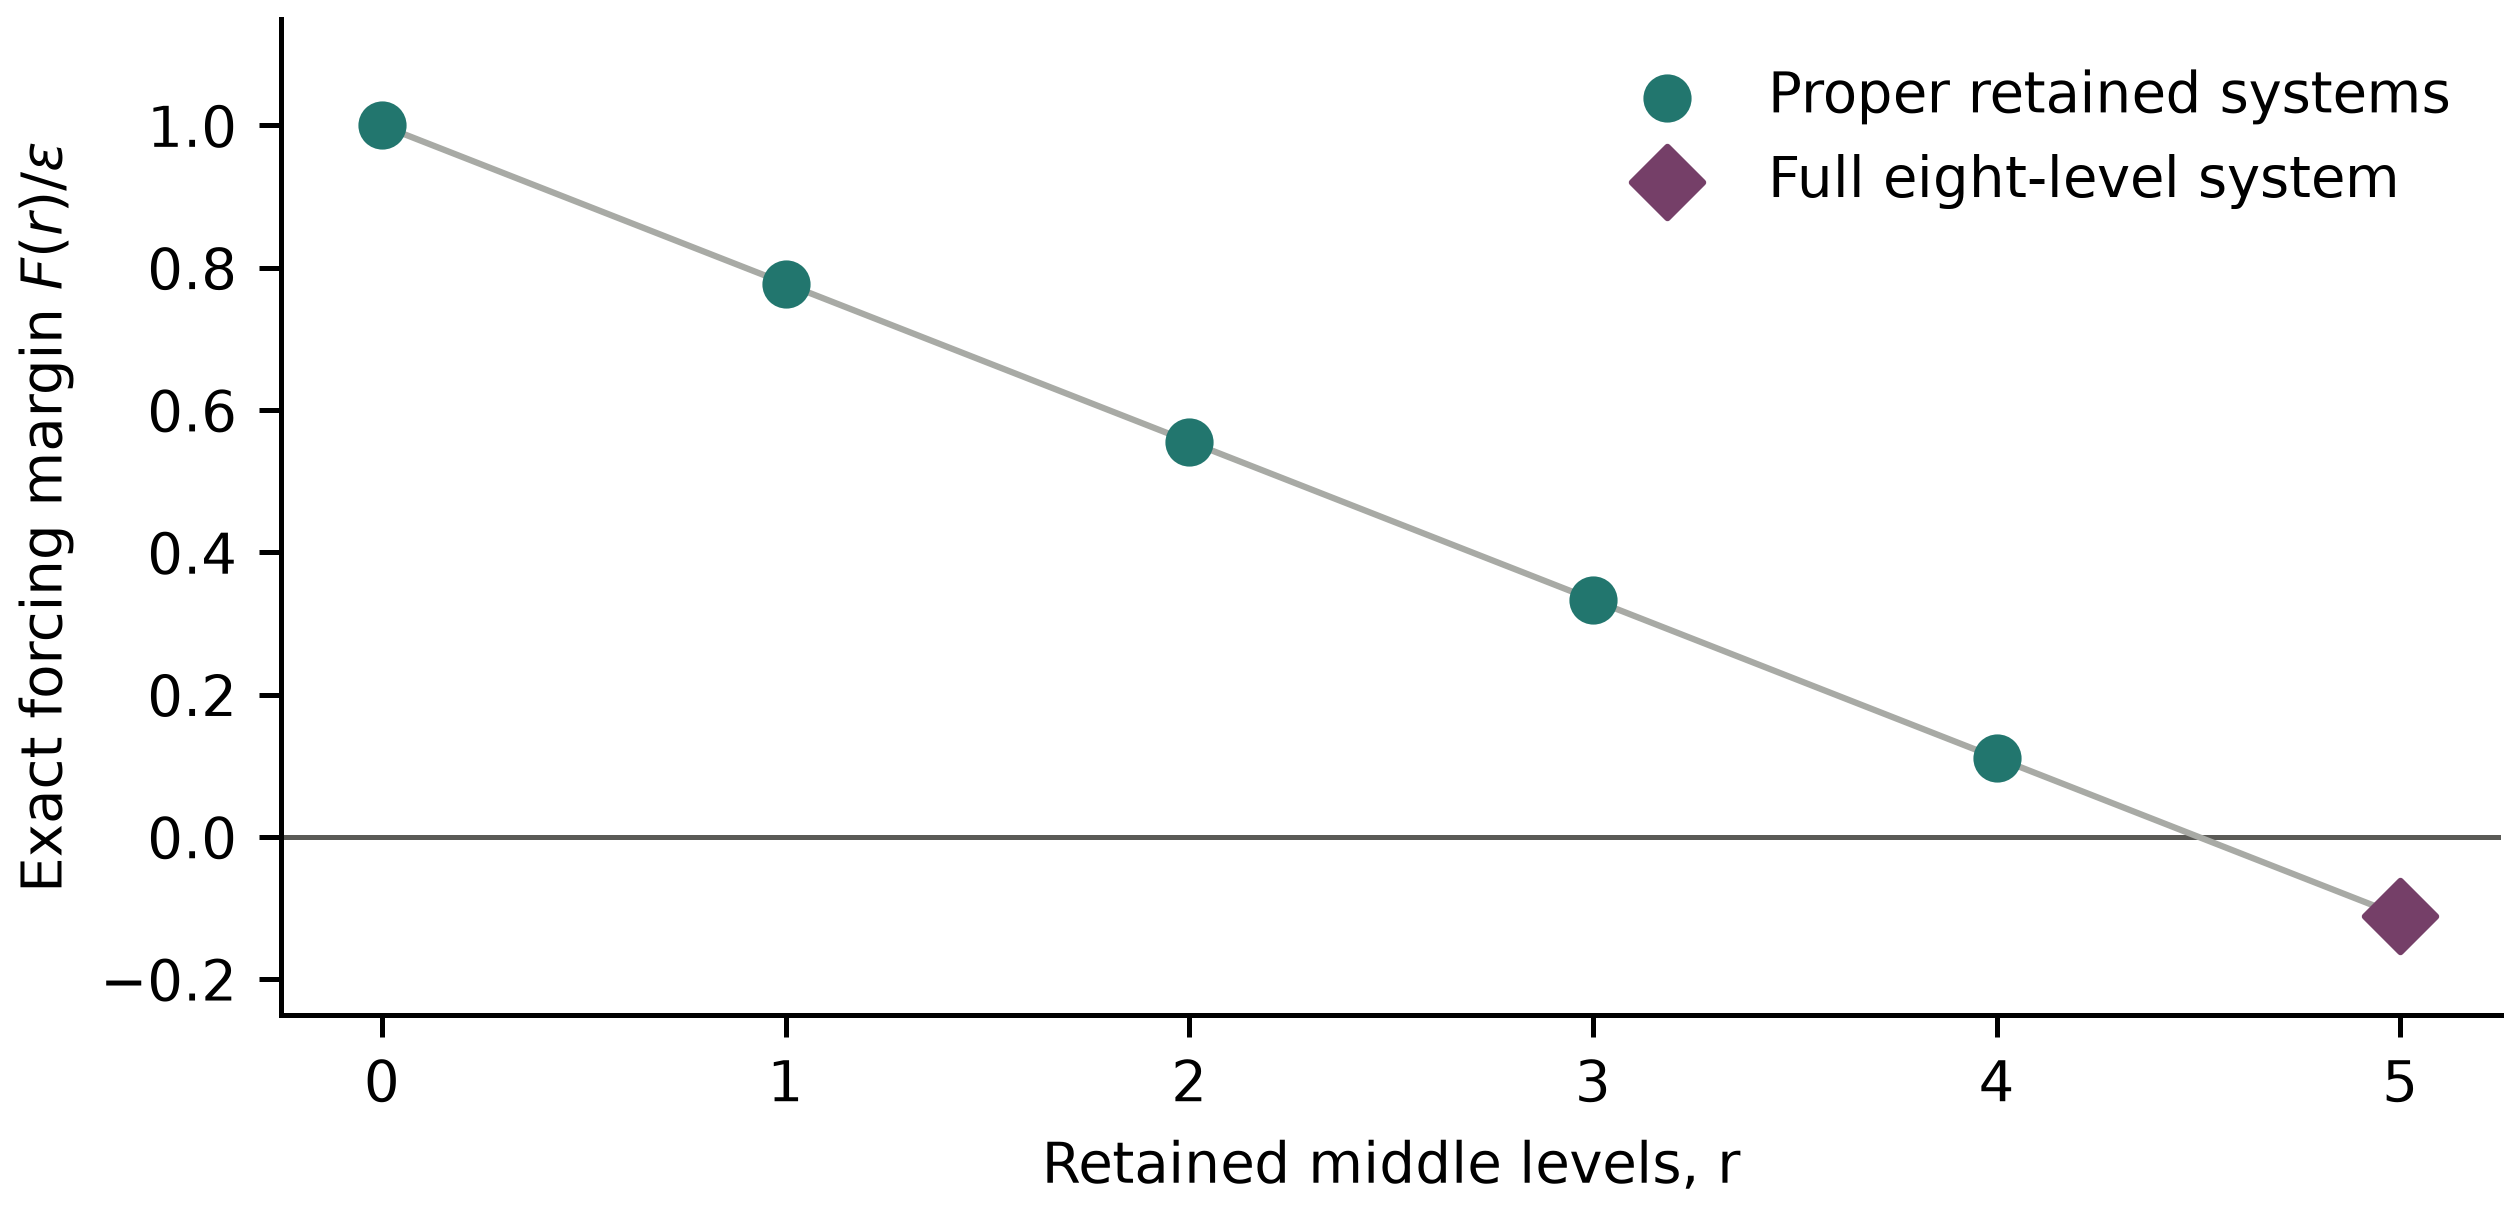
\includegraphics[width=.88\linewidth]{figures/hierarchy_margin.png}
\caption{A sign comparison that every proper restriction misses. For $N=8$ and $m=5$, the normalised forcing $F(r)/\varepsilon=1-r/(m-1/2)$ is positive for every proper restriction retaining the ground, slow state and top, and negative when all five middle levels are retained. Other types of proper subsystem are covered by Appendix~\ref{app:proper}. The connecting line visualises the exact affine formula, not an interpolation model for measured data.}
\label{fig:hierarchy}
\end{figure}

\subsection{A full-system cooling inversion}
Set $\varepsilon=1/100$ and define
\begin{equation}
 P_m=196m^2+294m-199,\qquad
 \theta_m=\frac{2m+3}{3(m+2)}-\frac1{(m+2)P_m}.
\end{equation}
Choose
\begin{equation}
 E=(0,1,2,\ldots,m+1,L),\qquad
 L>\frac{m+1}{2}+\frac{P_m(m+3)^2}{6}.
 \label{eq:L}
\end{equation}
Here $\theta_m$ is $\theta_r$ at $r=m$ with $\varepsilon=1/100$, since $100(2m-1)(C+mz)=P_m$. For the full slow amplitude $a(\beta)=p_\beta^Tg$, direct differentiation at the uniform preparation (Appendix~\ref{app:derivations}) gives
\begin{equation}
 a'(0)=\frac{L-(m+1)/2-P_m(m+3)^2/6}{P_m(m+3)^2}>0.
 \label{eq:Aprime}
\end{equation}
Hence there are finite $0<\beta_h<\beta_c$ with $0<a(\beta_h)<a(\beta_c)$. Initially the hotter preparation has smaller ground probability and larger total variation from the absorbing equilibrium. At late times Eq.~\eqref{eq:slow} reverses that order. Both amplitudes are nonzero, so this is ordinary inversion, not removal of the slow decay exponent.

\subsection{Simultaneous continuation to a finite bath}
Fix $N$, the spectrum in Eq.~\eqref{eq:L}, and two inverse temperatures in the increasing-amplitude interval. Keep every downward rate fixed and set
\begin{equation}
 a_{ji}(q)=a_{ij}q^{E_j-E_i},\qquad i<j,\quad q=e^{-\beta_b}>0.
 \label{eq:finitebath}
\end{equation}
Every off-diagonal rate is then positive, and every induced subsystem has the restricted, renormalised Gibbs equilibrium at the same bath.

At $q=0$, all subsystem spectra are simple. Normalise each slow eigenfunction as in Theorem~\ref{thm:hierarchy}(ii), so that the difference between its lowest two components is one; that difference is nonzero at $q=0$. Simple eigenpairs continue continuously as $q\downarrow0$. Each proper subsystem has finitely many strictly positive prefix margins, proved in Appendix~\ref{app:proper}; for fixed $N$ there are only finitely many subsystems. Let $\mu_N>0$ be the minimum, over the finite family of proper subsystems, of all their slow prefix margins and all gaps between distinct eigenvalues of each subsystem at $q=0$. Each of these finitely many quantities is continuous in $q$ at $q=0$ (simple eigenpairs of a matrix depending continuously on $q$), so each stays above $\mu_N/2$ for $0<q<q_S$ with some $q_S>0$. Taking $q_0(N)$ to be the minimum of the finitely many $q_S$ gives a common $q_0(N)>0$ that preserves all those margins and all spectral gaps for $0<q<q_0(N)$. Every genuine nonzero eigenfunction has stationary mean zero. Lemma~\ref{lem:gibbs} makes its Gibbs amplitude strictly decreasing for \emph{every} finite $\beta\ge0$, with its only zero at $\beta_b$. This conclusion uses finitely many margins, not a nonuniform continuity argument over unbounded preparation temperatures.

The chosen full-system amplitude inversion and initial total-variation inequality also persist. Taking $q$ smaller if necessary makes $\beta_b>\beta_c$, so both preparations cool. The slow-mode expansion supplies a late-time reversal and a finite crossing. All conditions used are strict and finite in number at the chosen positive bath. They persist under sufficiently small perturbations of the independent downward rates, with upward rates assigned by detailed balance. This proves Theorem~\ref{thm:hierarchy}. The argument is existential; it does not produce an explicit $q_0(N)$.

The continuation gives no bath threshold uniform in $N$ and does not preserve the zero-bath all-time total-variation assertion for every proper subsystem. At a finite bath the proved local conclusion is about the signed slow amplitude.

\begin{remark}[A certified four-level finite-bath instance]\label{rem:hier4}
For $N=4$ ($m=1$, $\varepsilon=1/100$, so $C=199/100$ and $z=23/25$), energies $E=(0,1,2,1555)$, which satisfy Eq.~\eqref{eq:L}, the bath $q=e^{-\beta_b}=1/1000$ ($\beta_b\approx6.91$) and the cooling preparations $e^{-\beta_h}=1-10^{-5}$, $e^{-\beta_c}=1-2\times10^{-5}$, the conclusions (i) and (ii) of Theorem~\ref{thm:hierarchy} are certified by exact rational and rational-interval arithmetic. All rates are positive and detailed balance holds exactly. Each of the six two-state and four three-state induced subsystems has simple spectrum and strictly positive slow prefix margins. The full generator has simple spectrum, with eigenvalues near $-3.91$, $-2.500667\ldots$ and $-1.001334\ldots$, each enclosed in a certified rational bracket of width below $10^{-70}$ (the first bracket ends at $-3.91$ itself, which is not an exact root); the brackets are disjoint, so the spectrum is simple, and slow amplitudes $0<a(\beta_h)<a(\beta_c)$ with ratio exceeding $1+3.37\times10^{-6}$. The total-variation gap $\TV(p_{\beta_h},\pi)-\TV(p_{\beta_c},\pi)$ is $+9.6244\times10^{-4}$ at $t=0$ and $-8.369018220250121\ldots\times10^{-11}$ at $t=10$ (both rational endpoints share these digits), so a crossing is certified in $(0,10)$. The same certificate also passes at $q=1/100$, but only on a knife edge.

This is a certified instance at one bath temperature, not an explicit $q_0(4)$: no interval of $q$ is certified, and a monotonicity or perturbation bound over $q\in(0,q_1]$ was not attempted. The binding constraint is the ground--slow--top triple $\{1,2,N\}$, which has the same rates for every $N$. Exact expansion of Eq.~\eqref{eq:helmert} gives
\begin{equation}
 H_{32}=\frac{\varepsilon-q}{2}+\frac{q^{L-1}(1-Cq)}{4},\qquad
 H_{23}=q^{L-1}(1-Cq),\qquad L=E_N,
 \label{eq:q0triple}
\end{equation}
so that triple's slow margin is positive if and only if $q<q^*=\varepsilon+O(\varepsilon^{L-1})$. The certificate fails at $q=1/10$, $1/20$ and $1/50$; at $q=1/50$ a 50-digit evaluation (numerical, not interval-certified) shows that the triple itself has an amplitude rise, i.e.\ a genuine local anomaly. Hence this construction needs $q\lesssim\varepsilon$, that is $\beta_b\gtrsim\log(1/\varepsilon)$, for every $N$. Together with the smallest upward rate, about $2\times10^{-4665}$ at $q=1/1000$ (top-to-ground gap $1555$), this shows how far the construction is from experimentally accessible scales.
\end{remark}

\subsection{What the hierarchy does and does not establish}
There is no fixed integer $k$ such that every slow-mode thermal anomaly has an anomalous induced subsystem with at most $k$ levels. This is a statement about retained-state anomaly witnesses. It does not prevent global inference from local rate data: all pair restrictions together determine the full generator.

The hierarchy also has an important reduction. At zero bath temperature the partition into ground, slow, all middle, and top states is strongly lumpable. Its four-block column generator is
\begin{equation}
 \overline M_r=\begin{pmatrix}
 0&1&3/2&C\\0&-1&1&1\\0&0&-5/2&rz\\0&0&0&-(C+1+rz)
 \end{pmatrix}.
 \label{eq:lump}
\end{equation}
Removing middle levels changes their aggregate Gibbs weight and the rate $rz$. Thus an unbounded minimal induced-level witness does not require an unbounded number of essential survival modes. For the explicit construction, the full prefix deficit is $O(N^{-3})$ and the sufficient top-energy scale in Eq.~\eqref{eq:L} is $O(N^4)$. These are not proved optimal bounds and do not establish experimental accessibility. Distinct middle energies generally break exact lumpability at a positive bath.

\section{Discussion}\label{sec:discussion}
The principal physical conclusion is the all-time ordering of excess free energy and the stated divergence family for concave jump weights, including common changes of those weights during relaxation. It requires no diagonalisation and no spectral simplicity hypothesis. Proposition~\ref{prop:baths} turns the condition into explicit cutoff thresholds for standard bath spectral densities, and Proposition~\ref{prop:superohmic} shows that a super-Ohmic weight can produce a real relative-entropy crossing. Concavity exactly characterises the universal cone criterion; it does not characterise the existence of crossings in general, since a nonconcave weight need not produce a crossing for a given spectrum. The super-Ohmic example shows only that leaving the concave class can have real consequences. The subsystem hierarchy establishes a different limit: the absence of slow-mode anomalies in every proper induced restriction does not certify the full system.

\subsection{Scope and limits}\label{sec:scope}
We collect here the limits stated in the body.
\begin{itemize}
\item \emph{Model class.} The physical class assumes a finite classical population process, a complete transition graph and a common pairwise coupling, Eq.~\eqref{eq:boson}. It excludes arbitrary state-dependent matrix elements, coherent quantum evolution, changing energies, changing bath temperatures and negative-temperature preparations. Sparse graphs such as the harmonic ladder or birth--death chains with nearest-neighbour transitions are not covered; whether an analogous classification holds there is open.
\item \emph{Sufficiency, not necessity, for crossings.} Theorem~\ref{thm:metric} is sufficient only. Failure of cone preservation does not by itself produce a crossing. The necessity direction of Theorem~\ref{thm:concavity} is about the cone, is existential over spectra, and uses many levels and cold baths jointly; at fixed $N$ or fixed $\beta_b$ concavity is not necessary.
\item \emph{Divergences.} The theorem covers the families in Table~\ref{tab:metrics}; it does not assert thermomajorization. Total variation is not covered, and Proposition~\ref{prop:TV} shows that it can reverse in the abstract cone-preserving class. That example lies outside the physical concave-$J$ class; whether finite-bath total variation is always ordered for concave $J$ is open (at zero bath it is, Sec.~\ref{sec:separators}). Whether the R\'enyi and power-divergence ranges are maximal is also open.
\item \emph{Baths and conventions.} The bath results apply to the jump weight $J$ of Eq.~\eqref{eq:boson}; a named spectral density must first be translated through the coupling convention (Sec.~\ref{sec:baths}). We do not claim that the class of reference~\cite{Avitan2026} equals the concave class.
\item \emph{Certified versus numerical.} The finite-time signs in Propositions~\ref{prop:TV} and \ref{prop:superohmic} and the statements of Remark~\ref{rem:hier4} are rational-interval certificates. Crossing locations from high-precision scans, slow-mode amplitudes in the super-Ohmic example, the triple anomaly at $q=1/50$, and the fixed-$(N,\beta_b)$ search for $J=1+d^2$ are numerical only.
\item \emph{Hierarchy.} The finite-bath part of Theorem~\ref{thm:hierarchy} is existential, with no explicit $q_0(N)$ and no threshold uniform in $N$. The construction requires $\beta_b\gtrsim\log(1/\varepsilon)$, a top energy of order $N^4$ and extremely small upward rates; it is not a proposal for an experiment. The no-fixed-$k$ statement concerns retained-state anomaly witnesses. It does not prevent global inference from local rate data, since all pair restrictions together determine the full generator, and it does not refute the three-level necessary conditions of reference~\cite{Avitan2026}. At zero bath the construction reduces exactly to four lumped blocks.
\item \emph{Prior art.} The literature comparison identifies prior statements and special-case collisions, including the slow-mode bath exclusion of reference~\cite{Avitan2026}, the Metropolis chain, the KL covariance calculation and the general invariant-cone method. It found no exact earlier statement of the combination proved here within the searched sources. This is a bounded prior-art assessment, not a proof of historical priority.
\end{itemize}

\section*{Reproducibility and provenance}
This version (1.0.0-candidate) and its research package are dated 28 October 2026 and archived at \href{https://doi.org/10.5281/zenodo.23721564}{doi:10.5281/zenodo.23721564}, with the repository at \url{https://github.com/ipitchford/thermal-ordering-concave-baths}; a SHA-256 manifest pins the delivered files. The bundle contains the manuscript source, figure scripts and data, exact checkers and outputs, an independent audit, a prior-art summary, the extension certificates in \texttt{extensions/}, and an isolated reproduction runner. The unrestricted statements rest on the proofs, while finite computations audit formulas, signs and conventions. None of the curves or searches is presented as experimental data.

From the bundle root, \texttt{python3 run\_checks.py} reproduces the default set without overwriting the retained outputs: four core exact checks and four extension certificates, all using only Python's standard library and compared exactly with the retained results. The physical formula checker passes 5,859 exact assertions over 96 rational models, including separate comparisons of $H^S$, $H^W$ and the directly transformed generator. The finite-operator checker uses rational stochastic uniformisation steps to audit the two adjoints and composition inequalities exactly; the semigroup and arbitrary-duration conclusions follow analytically. The hierarchy checker reconstructs slow eigenvectors in all 8,086 proper subsets for $N=4,\ldots,12$ at $\varepsilon=1/100$, plus 1,368 subsets at other parameter values; its all-time checks concern the signs of coefficients and endpoint expressions in the proof, rather than sampled times. The extension certificates reproduce the threshold audit of Proposition~\ref{prop:baths}, the certificate of Proposition~\ref{prop:superohmic}, Remark~\ref{rem:hier4}, and Table~\ref{tab:prop5cert} with its perturbation checks. The optional \texttt{--independent} flag adds a separately implemented floating-point audit (2,871 subsystem checks, 80 rational concave-kernel models and noncommuting finite-time comparisons), compared with relative tolerance $10^{-9}$ and absolute tolerance $10^{-12}$. Optional high-precision positive-bath illustrations are not interval certificates; one such four-state example at $\beta_b=10$ has a computed TV difference changing from about $9.6243\times10^{-4}$ at time zero to $-7.3692\times10^{-11}$ at time 10, with smallest upward rate about $10^{-6753}$. \texttt{manuscript/make\_figures.py} regenerates the illustrations, using NumPy, SciPy and Matplotlib.

Research and verification were AI-assisted (see the note on the title page). The manuscript has not undergone external specialist peer review, and no journal acceptance or publication priority is implied by the internal checks. No individual author or institutional affiliation is assigned.

\appendix
\section{The rational finite-time certificate}\label{app:certificate}
Here is a complete finite prescription for Eqs.~\eqref{eq:tvinit}--\eqref{eq:tvfinal}. All inputs in Eq.~\eqref{eq:tvG}, the two populations $p_3,p_4$, and $t_*=1047/100$ are rational. Choose uniformisation rate $R=2$, set $P=I+G/R$ and $x=Rt_*=1047/50$. Direct rational checks give $P_{ij}\ge0$ and $P\one=\one$. For a row population $p^T$, define
\begin{equation}
 S_i=\sum_{k=0}^{100}\frac{x^k}{k!}(p^TP^k)_i,\qquad
 B=\sum_{k=0}^{100}\frac{x^k}{k!},\qquad
 T=\frac{x^{101}}{101!}\frac1{1-x/102}.
 \label{eq:certificate}
\end{equation}
The exponential tail is bounded by a geometric series, since every successive ratio after the first omitted term is at most $x/102<1$. Thus
\begin{equation}
 B\le e^x\le B+T,\qquad
 \frac{S_i}{B+T}\le(p^Te^{t_*G})_i\le\frac{S_i+T}{B}.
 \label{eq:interval}
\end{equation}
The second bound uses $0\le(p^TP^k)_i\le1$ term by term. No approximation of the matrix exponential enters these inequalities.

For each preparation, compare these rational endpoints with the rational $\pi_i$. The intervals for components $1,2,4$ lie strictly above $\pi_i$, and those for components $3,5$ lie strictly below. Since $\TV(p,\pi)=\sum_{i:p_i>\pi_i}(p_i-\pi_i)$, the equilibrium terms cancel when subtracting the two preparations on their common positive set. A lower bound on the final difference is the sum of the warm lower endpoints minus the cold upper endpoints over $\{1,2,4\}$; the reverse endpoint choice gives the upper bound. Comparing those fractions with the rational decimal endpoints in Eq.~\eqref{eq:tvfinal} proves the displayed signs. At $t=10.46$ and $t=10.48$ the two preparations have different certified positive sets; the same argument is then applied to each preparation separately, bounding $\TV(p_\beta(t),\pi)$ below by the sum of its lower endpoints minus $\pi_i$ over its own positive set and above by the corresponding upper endpoints, which gives Eq.~\eqref{eq:tvbrackets}. Direct rational evaluation gives Eq.~\eqref{eq:tvinit}. The script \texttt{metric\_sharpness/certify\_counterexamples.py} implements precisely this prescription and also checks detailed balance and Eq.~\eqref{eq:tvH}. The script \texttt{extensions/c1\_prop5\_certificate.py} repeats it at $t=10.46,10.47,10.48$ and for the perturbed models, and writes the exact endpoints summarised in Table~\ref{tab:prop5cert}.

\section{All proper subsystems in the hierarchy}\label{app:proper}
Write $r$ for the number of retained middle states. Which middle labels are retained does not affect the reduced rates after reindexing. At zero bath temperature the equilibrium is the least retained state. Its survival response is zero; all other responses initially equal one. The following four classes exhaust every retained-state set. Singletons have no nonzero mode, and every two-state case is conventional.

\subsection{Both distinguished low states retained}
Here $r$ is the number of retained middle states. If the top is present and the subsystem is proper, then $r\le m-1$. The middle survival responses are all $h_M=(2/3)e^{-t}+(1/3)e^{-5t/2}$ because their mutual transitions cancel when the responses agree. This follows either by substitution into the backward equations with the shared initial value or by induction in retained energy order. Each middle prefix comparison is positive because
\begin{equation}
 2h_M-h_2=\tfrac13e^{-t}+\tfrac23e^{-5t/2}>0.
\end{equation}
When the top is retained, Eq.~\eqref{eq:survivalforcing} proves the last comparison. Without the top there is no further comparison. The corresponding slow response is Eq.~\eqref{eq:hierg}, with the last coordinate omitted when necessary, and has strictly positive prefix margins. The escape rates are $1$, then $5/2+s\delta$ for successive $s\ge0$, then $C+1+rz$ if the top is present. The top rate exceeds all preceding ones by $C>3/2$ and $z>\delta$.

\subsection{Ground retained, slow state removed}
Here $r$ is the number of retained middle states. For $r\ge1$ every middle survival response is $e^{-3t/2}$. If the top is present, put $\Gamma=C+rz>3/2$ and
\begin{equation}
 b=\frac{rz}{C+rz-3/2},\qquad
 h_N(t)=be^{-3t/2}+(1-b)e^{-\Gamma t}.
\end{equation}
Subtracting the preceding prefix mean gives
\begin{equation}
 e^{-3t/2}\left[b-\frac{r}{r+1}+(1-b)e^{-(\Gamma-3/2)t}\right].
\end{equation}
The bracket is affine in a variable in $[0,1]$. Its endpoint values are $1/(r+1)$ and
\begin{equation}
 b-\frac{r}{r+1}
 =\frac{r(z-C+3/2)}{(r+1)(C+rz-3/2)}>0.
\end{equation}
All other prefix comparisons are immediate. The slow response $(0,1,\ldots,1,b)$ has the same strict comparisons. With no top the conclusion follows from equal excited responses. The middle escape rates are $3/2+s\delta$ and the top rate is larger by Eq.~\eqref{eq:paramineq}.

\subsection{Slow state retained, ground removed}
Here $r$ is the number of retained middle states. State 2 becomes the subsystem ground. Every other retained state has direct absorption rate one into it, so all excited survival responses are exactly $e^{-t}$ irrespective of their mutual transitions. The slow response $(0,1,\ldots,1)$ has strictly increasing prefix means. Middle escape rates are $1+s\delta$, and the optional top rate $1+rz$ exceeds them because $z>\delta$.

\subsection{Both distinguished low states removed}
Here $r$ is the number of retained middle states \emph{including} the least one, which becomes the subsystem ground, so the top rate $rz$ below counts all of them. If $r\ge2$, the least retained middle is the ground and every other middle has direct absorption rate $\delta$. Their survival responses equal $e^{-\delta t}$. If the top is present, its escape rate is $rz>\delta$, and
\begin{equation}
 h_N(t)=be^{-\delta t}+(1-b)e^{-rzt},\qquad
 b=\frac{(r-1)z}{rz-\delta}.
\end{equation}
The final prefix comparison is positive by the same affine-endpoint argument, with endpoints $1/r$ and
\begin{equation}
 b-\frac{r-1}{r}=\frac{(r-1)\delta}{r(rz-\delta)}>0.
\end{equation}
The corresponding slow response has middle values one and top value $b$, and all its prefix margins are strict. Without the top, all excited responses agree. With one middle and the top, the system is two-state. The middle escape rates are $\delta,2\delta,\ldots,(r-1)\delta$, and $rz$ exceeds all of them.

For each class, the survival vector lies in $\C$ at every finite time. Its Gibbs average equals total variation from the absorbing ground, so Lemma~\ref{lem:gibbs} proves the all-time local statement. The explicitly strict slow-prefix margins also supply the finite collection of inequalities used in the positive-bath continuation.

\section{Derivations of the main matrix formulas}\label{app:derivations}
\paragraph{The quotient, Eq.~\eqref{eq:helmert}.} Since $(u^{(i)})^Tx=(i-1)d_i(x)$ and $G\one=0$, expanding $b$ in the orthogonal contrasts gives $d_i(Gb)=(u^{(i)})^TGb/(i-1)=\sum_j(u^{(i)})^TGu^{(j)}d_j(b)/[(i-1)j]$.

\paragraph{The thermal part, Eq.~\eqref{eq:thermalH}.} For the symmetric generator $S$ with off-diagonal entries $s_{k\ell}=h(|E_k-E_\ell|)$, $x^TSy=-\sum_{k<\ell}s_{k\ell}(x_k-x_\ell)(y_k-y_\ell)$. Take $x=u^{(i)}$, $y=u^{(j)}$ with $i<j$. Pairs with both indices below $j$ have $y_k=y_\ell$ unless $\ell=j$, and pairs with both indices above $i$ have $x_k=x_\ell=0$. The surviving pairs are $(k,j)$ with $k\le i$, contributing $j\,s_{kj}(x_k-x_j)$, and $(k,\ell)$ with $k\le i<j<\ell$, contributing $-s_{k\ell}(x_k-x_\ell)(y_k-y_\ell)$ with $y_k-y_\ell=-1$. Using $x_k=-1$ for $k<i$ and $x_i=i-1$,
\begin{equation}
 (u^{(i)})^TSu^{(j)}=j\Big[(i-1)h(E_j-E_i)-\sum_{k<i}h(E_j-E_k)\Big]+\sum_{\ell>j}\Big[(i-1)h(E_\ell-E_i)-\sum_{k<i}h(E_\ell-E_k)\Big].
\end{equation}
Dividing by $(i-1)j$ gives Eq.~\eqref{eq:thermalH}. Each bracket is nonnegative because $h$ is nonincreasing and $E_j-E_i<E_j-E_k$ for $k<i$. Symmetry of $S$ gives the relation between $H^S_{ji}$ and $H^S_{ij}$.

\paragraph{The emission part, Eq.~\eqref{eq:downH}.} For $W$, $(Wx)_k=\sum_{\ell<k}J(E_k-E_\ell)(x_\ell-x_k)$. Hence $(Wu^{(j)})_k=0$ for $k<j$, $(Wu^{(j)})_j=-jS_j$, and $(Wu^{(j)})_k=F_j(E_k)$ for $k>j$. Since $u^{(i)}$ is supported on indices at most $i$, $(u^{(i)})^TWu^{(j)}=0$ for $i<j$. For $i>j$,
\begin{equation}
 (u^{(i)})^TWu^{(j)}=jS_j-\sum_{k=j+1}^{i-1}F_j(E_k)+(i-1)F_j(E_i),
\end{equation}
which rearranges to Eq.~\eqref{eq:downH}. $F_j$ is nondecreasing because $F_j(x)=-\sum_{\ell<j}I_{E_j-E_\ell}(x-E_j)$ and each increment is nonincreasing by Lemma~\ref{lem:increments}.

\paragraph{The necessity limit, Eq.~\eqref{eq:necessity}.} Take $j=2$, $i=N=M+3$ and energies $0,\Delta$, $M$ levels at (the limit) $\Delta+x$, and $\Delta+y$. Then $S_2=J(\Delta)$, $F_2(E_N)=J(y)-J(\Delta+y)=-I_\Delta(y)$ and $F_2(E_k)\to-I_\Delta(x)$ for the middle levels. Equation~\eqref{eq:downH} gives $2(M+2)H^W_{N2}\to2[J(\Delta)-I_\Delta(y)]+M[I_\Delta(x)-I_\Delta(y)]$, which is Eq.~\eqref{eq:necessity}.

\paragraph{The amplitude slope, Eq.~\eqref{eq:Aprime}.} By Lemma~\ref{lem:gibbs}, $a'(0)=-\Cov_u(E,g)$ for the uniform distribution $u$ on the $N=m+3$ states. Write $g=g^0-[(m+2)P_m]^{-1}e_N$, where $g^0=(0,1,2/3,\ldots,2/3,(2m+3)/(3(m+2)))$ and $e_N$ is the top indicator. With $E=(0,1,2,\ldots,m+1,L)$, direct summation gives $\Cov_u(E,g^0)=1/6$, independent of $L$, and $\Cov_u(E,e_N)=(m+2)[L-(m+1)/2]/(m+3)^2$. Therefore
\begin{equation}
 a'(0)=-\frac16+\frac{L-(m+1)/2}{P_m(m+3)^2},
\end{equation}
which is Eq.~\eqref{eq:Aprime}.

\begin{thebibliography}{99}\raggedright
\bibitem{LuRaz2017}
Z. Lu and O. Raz, Nonequilibrium thermodynamics of the Markovian Mpemba effect and its inverse, \emph{Proc. Natl. Acad. Sci. USA} \textbf{114}, 5083--5088 (2017). \url{https://doi.org/10.1073/pnas.1701264114}.
\bibitem{Klich2019}
I. Klich and M. Vucelja, Mpemba effect on near-complete graphs with independence Metropolis--\allowbreak Hastings dynamics, \emph{J. Phys. A: Math. Theor.} \textbf{59}, 255002 (2026); preprint arXiv:1812.11962 (2018) under the title ``Solution of the Metropolis dynamics on a complete graph with application to the Markov chain Mpemba effect''. \url{https://doi.org/10.1088/1751-8121/ae7228}.
\bibitem{Ohga2024}
N. Ohga, H. Hayakawa, and S. Ito, Microscopic theory of Mpemba effects and a no-Mpemba theorem for monotone many-body systems, arXiv:2410.06623v2 (2024). \url{https://arxiv.org/abs/2410.06623v2}.
\bibitem{Avitan2026}
I. Avitan, R. Factor, and D. Gelbwaser-Klimovsky, Necessary conditions for the Markovian Mpemba effect, arXiv:2603.04567v1 (2026). \url{https://arxiv.org/abs/2603.04567v1}.
\bibitem{Gelbwaser2026}
D. Gelbwaser-Klimovsky, Efficient protocol for the Markovian Mpemba effect in $N$-level systems, arXiv:2609.09988v1 (2026). \url{https://arxiv.org/abs/2609.09988v1}.
\bibitem{Biernacki1951}
M. Biernacki, Sur une in\'egalit\'e entre les int\'egrales due \`a Tch\'ebyscheff, \emph{Annales Universitatis Mariae Curie-Sk\l odowska, Sectio A} \textbf{5}, 23--29 (1951). \url{https://bc.umcs.pl/Content/30587/PDF/czas4050_5_1951_2.pdf}.
\bibitem{Dragomir2004}
S. S. Dragomir, New Chebyshev type inequalities for sequences of real numbers, \emph{Rev. Anal. Num\'er. Th\'eor. Approx.} \textbf{33}(1), 61--66 (2004). \url{https://ictp.acad.ro/jnaat/journal/article/download/2004-vol33-no1-art7/759}.
\bibitem{Lorek2012}
P. Lorek and R. Szekli, Strong stationary duality for M\"obius monotone Markov chains, \emph{Queueing Systems} \textbf{71}, 79--95 (2012). \url{https://doi.org/10.1007/s11134-012-9284-z}.
\bibitem{Vu2025}
T. Van Vu and H. Hayakawa, Thermomajorization Mpemba Effect, \emph{Phys. Rev. Lett.} \textbf{134}, 107101 (2025). \url{https://doi.org/10.1103/PhysRevLett.134.107101}.
\bibitem{Summer2026}
A. Summer, M. Moroder, L. P. Bettmann, X. Turkeshi, I. Marvian, and J. Goold, Resource-Theoretical Unification of Mpemba Effects: Classical and Quantum, \emph{Phys. Rev. X} \textbf{16}, 011065 (2026). \url{https://doi.org/10.1103/rbt4-psfd}.
\bibitem{Salazar2026}
D. S. P. Salazar, Divergence Geometry of Quantum Multi-Mpemba Effects, arXiv:2609.20320v2 (2026). \url{https://arxiv.org/abs/2609.20320v2}.
\bibitem{Wang2026}
Y. Wang and Z. Lu, Slow is fast: raising barriers to accelerate thermal relaxation, arXiv:2607.11877v1 (2026). \url{https://arxiv.org/abs/2607.11877v1}.
\bibitem{Cressie1984}
N. Cressie and T. R. C. Read, Multinomial Goodness-of-Fit Tests, \emph{J. R. Stat. Soc. B} \textbf{46}, 440--464 (1984). \url{https://doi.org/10.1111/j.2517-6161.1984.tb01318.x}.
\bibitem{Hiai2017}
F. Hiai, M. Mosonyi, D. Petz, and C. B\'eny, Quantum $f$-divergences and error correction, \emph{Rev. Math. Phys.} \textbf{23}, 691--747 (2011); arXiv:1008.2529v6 (revised 2017). \url{https://doi.org/10.1142/S0129055X11004412}.
\bibitem{KlichRaz2019}
I. Klich, O. Raz, O. Hirschberg, and M. Vucelja, Mpemba Index and Anomalous Relaxation, \emph{Phys. Rev. X} \textbf{9}, 021060 (2019). \url{https://doi.org/10.1103/PhysRevX.9.021060}.
\bibitem{Kumar2020}
A. Kumar and J. Bechhoefer, Exponentially faster cooling in a colloidal system, \emph{Nature} \textbf{584}, 64--68 (2020). \url{https://doi.org/10.1038/s41586-020-2560-x}.
\bibitem{Walker2021}
M. R. Walker and M. Vucelja, Anomalous thermal relaxation of Langevin particles in a piecewise-constant potential, \emph{J. Stat. Mech.: Theory Exp.} \textbf{2021}, 113105 (2021). \url{https://doi.org/10.1088/1742-5468/ac2edc}.
\bibitem{Lapolla2020}
A. Lapolla and A. Godec, Faster Uphill Relaxation in Thermodynamically Equidistant Temperature Quenches, \emph{Phys. Rev. Lett.} \textbf{125}, 110602 (2020); Erratum, \emph{Phys. Rev. Lett.} \textbf{128}, 229901 (2022). \url{https://doi.org/10.1103/PhysRevLett.125.110602}, \url{https://doi.org/10.1103/PhysRevLett.128.229901}.
\bibitem{VanVu2021}
T. Van Vu and Y. Hasegawa, Toward relaxation asymmetry: Heating is faster than cooling, \emph{Phys. Rev. Res.} \textbf{3}, 043160 (2021). \url{https://doi.org/10.1103/PhysRevResearch.3.043160}.
\bibitem{Ibanez2024}
M. Ib\'a\~nez, C. Dieball, A. Lasanta, A. Godec, and R. A. Rica, Heating and cooling are fundamentally asymmetric and evolve along distinct pathways, \emph{Nat. Phys.} \textbf{20}, 135--141 (2024). \url{https://doi.org/10.1038/s41567-023-02269-z}.
\bibitem{Daley1968}
D. J. Daley, Stochastically monotone Markov chains, \emph{Z. Wahrscheinlichkeitstheorie verw. Gebiete} \textbf{10}, 305--317 (1968). \url{https://doi.org/10.1007/BF00531852}.
\bibitem{KeilsonKester1977}
J. Keilson and A. Kester, Monotone matrices and monotone Markov processes, \emph{Stoch. Process. Appl.} \textbf{5}, 231--241 (1977). \url{https://doi.org/10.1016/0304-4149(77)90033-3}.
\bibitem{Massey1987}
W. A. Massey, Stochastic Orderings for Markov Processes on Partially Ordered Spaces, \emph{Math. Oper. Res.} \textbf{12}, 350--367 (1987). \url{https://doi.org/10.1287/moor.12.2.350}.
\bibitem{Shaked2007}
M. Shaked and J. G. Shanthikumar, \emph{Stochastic Orders}, Springer Series in Statistics (Springer, New York, 2007). \url{https://doi.org/10.1007/978-0-387-34675-5}.
\end{thebibliography}
\end{document}
